\documentclass[]{osa-article}

%% Select the journal you're submitting to
%% oe, boe, ome, osac, osajournal
\journal{osajournal}
% Key:
% Express journals must have the correct journal selected:
% {oe} Optics Express
% {boe} Biomedical Optics Express
% {ome} Optical Material Express
% {osac} OSAC Continuum
% Other OSA journals may use:
% {osajournal} Applied Optics, Advances in Optics and Photonics, Journal of the Optical Society of America A/B, Optics Letters, Optica, Photonics Research

% Uncomment if submitting to Photonics Research.
% ONLY APPLICABLE FOR \journal{osajournal}
% \setprjcopyright

% Set the article type
\articletype{Research Article}
% Note that article type is not required for Express journals (OE, BOE, OME and OSAC)

% Talon's custom libraries
\usepackage{empheq}
\usepackage{bm}

% Talon's custom commands
\setlength\arraycolsep{1.5pt}
\let\originalleft\left
\let\originalright\right
\renewcommand{\left}{\mathopen{}\mathclose\bgroup\originalleft}
\renewcommand{\right}{\aftergroup\egroup\originalright}
\DeclareMathAlphabet{\mathcal}{OMS}{cmsy}{m}{n}
\newcommand{\tensor}[1]{\overset{\text{\tiny$\leftrightarrow$}}{\mb{#1}}}
\newcommand{\argmin}{\arg\!\min}
\newcommand{\me}{\mathrm{e}}
\providecommand{\e}[1]{\ensuremath{\times 10^{#1}}} 
\providecommand{\mb}[1]{\mathbf{#1}}
\providecommand{\msf}[1]{\mathsf{#1}}
\providecommand{\mf}[1]{\mathfrak{#1}}
\providecommand{\mc}[1]{\mathcal{#1}}
\providecommand{\ro}{\mathbf{\mathbf{r}}_o}
\providecommand{\so}{\mathbf{\hat{s}}_o}
\providecommand{\rp}{\mathbf{r}_p}
\providecommand{\rbm}[1]{r_b^{\text{m}}}
\providecommand{\rd}{\mathbf{r}_d}
\providecommand{\rdf}{\mathpzc{r}_d}
\providecommand{\mh}[1]{\mathbf{\hat{#1}}}
\providecommand{\mbb}[1]{\mathbb{#1}}
\providecommand{\bs}[1]{\boldsymbol{#1}}
\providecommand{\bv}{\bs{\nu}}
\providecommand{\taup}{\bs{\tau}}
\providecommand{\bsh}[1]{\hat{\boldsymbol{#1}}}
\providecommand{\nan}{\left(\frac{\text{NA}}{n_o}\right)}
\providecommand{\lmsum}{\sum_{\ell=0}^\infty\sum_{m=-\ell}^{\ell}}
\providecommand{\intr}[1]{\int_{\mbb{R}^{#1}}}
\providecommand{\ints}[1]{\int_{\mbb{S}^{#1}}}
\providecommand{\tb}[1]{\textcolor{blue}{#1}}
% \DeclareFontFamily{OT1}{pzc}{}
% \DeclareFontShape{OT1}{pzc}{m}{it}{<-> s * [1.10] pzcmi7t}{}
% \DeclareMathAlphabet{\mathpzc}{OT1}{pzc}{m}{it}
\newcommand{\eqname}[1]{\tag*{#1}}
\newcommand*\widefbox[1]{\fbox{\hspace{1em}#1\hspace{1em}}}

\begin{document}

\title{Spatio-angular fluorescence microscopy\\ I. Basic theory}

\author{Talon Chandler,\authormark{1,*} Hari Shroff,\authormark{2,3} Rudolf Oldenbourg,\authormark{3} and Patrick La Rivi\`ere\authormark{1,3}}

\address{\authormark{1}University of Chicago, Department of Radiology, Chicago, Illinois 60637, USA\\
  \authormark{2}Section on High Resolution Optical Imaging, National Institute
  of Biomedical Imaging and Bioengineering, National Institutes of Health,
  Bethesda, Maryland 20892, USA\\
  \authormark{3}Marine Biological Laboratory, Bell Center, Woods Hole, Massachusetts 02543, USA
}

\email{\authormark{*}talonchandler@talonchandler.com} %% email address is required

%\homepage{talonchandler@talonchandler.com} %% author's URL, if desired

%%%%%%%%%%%%%%%%%%% abstract %%%%%%%%%%%%%%%%
%% [use \begin{abstract*}...\end{abstract*} if exempt from copyright]

\begin{abstract*}
  We introduce the basic elements of a spatio-angular theory of fluorescence
  microscopy. We start by modeling an aplanatic microscope imaging an ensemble
  of in-focus fluorescent dipoles as a linear Hilbert-space operator, and we
  show that the operator takes a particularly convenient form when expressed in
  a basis of complex exponentials and spherical harmonics---a form we call the
  dipole spatio-angular transfer function. We demonstrate our formalism by
  analyzing a single-view fluorescence microscope without using the monopole or
  scalar approximations. We show that this imaging system has a spatio-angular
  band limit, and we exploit the band limit to perform efficient simulations.
  Notably, we show that information about the out-of-plane orientation of
  ensembles of in-focus fluorophores is recorded by paraxial fluorescence
  microscopes.
\end{abstract*}

\section{Introduction}
Fluorescence microscopes are widely used in the biological sciences for imaging
fluorescent molecules that label specific proteins and biologically important
molecules. While most fluorescence microscopy experiments are designed to
measure only the spatial distribution of fluorophores, a growing number of
experiments seek to measure both the spatial and angular distributions of
fluorophores by the use of polarizers \cite{vrabioiu2006, mattheyses2010,
  mehta2016, mcquilken2017, zhanghao2017} or point spread function engineering
\cite{agrawal2012, zhang2018}.

Meanwhile, single-molecule localization microscopy (SMLM) experiments use
spatially sparse fluorescent samples to localize single molecules with precision
that surpasses the diffraction limit. Noise limits the precision of this
localization \cite{foreman2011, chao2016}, and several studies have shown that
model mismatch (e.g. ignoring the effects of vector optics, dipole orientation
\cite{backlund2014}, and dipole rotation \cite{lew2013}) can introduce
localization bias as well. Therefore, the most precise and accurate SMLM
experiments must use an appropriate model and jointly estimate both the position
and orientation of each fluorophore. Several studies have successfully used
vector optics and dipole models to estimate the position and orientation of
single molecules \cite{bohmer2003, lieb2004, toprak2006, aguet2009}, and there
is growing interest in designing optical systems for measuring the position,
orientation, and rotational dynamics of single molecules \cite{agrawal2012,
  backer2014, stallinga2015, zhang2018, zhang2018-2}.

While many studies have focused on improving imaging models for spatially sparse
fluorescent samples, we consider the more general case and aim to improve
imaging models for arbitrary samples including those containing ensembles of
fluorophores within a resolvable volume. In particular, we examine the effects
of two widely used approximations in fluorescence microscopy---the
\textit{monopole approximation} and the \textit{scalar approximation}.

We use the term \textit{monopole} to refer to a model of a fluorophore that
treats it as an isotropic absorber/emitter. Although the term \textit{monopole
  approximation} is not in widespread use, we think it accurately describes the
way many models of fluorescence microscopy treat fluorophores, and we use the
term to distinguish the monopole model from more realistic dipole and
higher-order models. Despite their use in models, electromagnetic monopole
absorber/emitters do not exist in nature. All physical fluorophores absorb and
emit radiation with dipole or higher-order moments, and these moments are always
oriented in space. For a classical mental model of fluorophores we imagine each
dipole as a small oriented antenna (with incoherent absorption and emission
moments) where electrons are constrained to move along a single direction. % With
% this model we can argue classically that monopole radiators do not exist because
% they would violate the conservation of charge.

Although many works implicitly apply the monopole approximation, we have
encountered two explicit justifications: (1) the sample contains many randomly
oriented fluorophores within a resolvable volume or (2) the sample contains
unconstrained rotating fluorophores. While both of these situations yield
monopole-like emitters, neither yields emitters that are perfectly described by
the monopole model. In this work we investigate the dipole model of fluorophores
in detail and find the conditions under which the monopole approximation is
justified.

All fluorescence microscopy models that use an \textit{optical point spread
  function} or an \textit{optical transfer function} to describe the mapping
between the fluorophores and the irradiance on the detector implicitly make the
monopole approximation. The optical point spread function is the irradiance
response of an optical system to an isotropic point source, so it cannot model
the response due to an anisotropic dipole radiator. In this work we define
\textit{monopole and dipole transfer functions} that describe the mapping
between fluorophores and the measured irradiance. Although optical systems are
an essential part of microscopes, fluorescence microscopists are interested in
measuring the properties of fluorophores (not optics), so the monopole and
dipole transfer functions are more directly useful than the optical transfer
function for the problems that fluorescence microscopists are interested in
solving.

While the monopole approximation applies to the fluorescent object, the
\textit{scalar approximation} applies to the fields that propagate through the
microscope. Modeling the electric fields in a region requires a
three-dimensional vector field, but if the electric fields are random or
completely parallel, a scalar field is sufficient, and we can replace the
vector-valued electric field, $\mb{E}$, with a scalar-valued field, $U$.

The scalar approximation is often made together with the monopole approximation.
For example, the Born-Wolf model \cite{born1980} and the Gibson-Lanni model
\cite{gibson89} make both the monopole and scalar approximations when applied to
fluorescence microscopes. However, some models make the monopole approximation
but not the scalar approximation. For example, the Richards-Wolf model
\cite{richards} considers the role of vector-valued fields in the optical
system, but it is an optical model so when it is applied to fluorescence
microscopes the monopole approximation is assumed. 

This work lies at the intersection of three subfields of fluorescence
microscopy: (1) spatial ensemble imaging where each resolvable volume contains
many fluorophores and the goal is to find the concentration of fluorophores as a
function of position in the sample, (2) spatio-angular ensemble imaging where
each resolvable volume contains many fluorophores and the goal is to find the
concentration and orientation of fluorophores as a function of position in the
sample, and (3) SMLM imaging where fluorophores are sparse in the sample and the
goal is to find the position and orientation of each fluorophore. We briefly
review how these three subfields use the monopole and scalar approximations.

The large majority of fluorescence microscopes are used to image ensembles of
fluorophores, and most existing modeling techniques make use of the monopole
approximation, the scalar approximation, or both. As discussed above, the
Gibson-Lanni model, the Born-Wolf model, and the Richards-Wolf model are
approximate when applied to fluorescence microscopy data because they only model
monopole emitters. Deconvolution algorithms that use these models may make
biased estimates of fluorophore concentrations since they ignore the dipole
excitation and emission of fluorophores, but we will see that these effects are
small when the sample contains many randomly oriented fluorophores within a
resolvable volume or unconstrained rotating fluorophores.

A small but growing group of microscopists is interested in measuring the
orientation and position of ensembles of fluorophores \cite{vrabioiu2006,
  mattheyses2010, mehta2016, mcquilken2017, zhanghao2017}. These techniques
typically use polarizers to make multiple measurements of the same object with
different polarizer orientations, then they use a model of the dipole excitation
and emission processes \cite{fourkas2001} to recover the orientation of
fluorophores using pixel-wise arithmetic. Although these studies do not adopt
the scalar or monopole approximations for the angular part of the problem, they
adopt both approximations when they consider the spatial part of the problem.
Existing works either ignore the spatial reconstruction problem
\cite{vrabioiu2006, mattheyses2010, mehta2016, mcquilken2017} or assume that the
spatial and angular reconstruction problems can be solved sequentially
\cite{zhanghao2017}.

The most precise experiments in SMLM imaging do not adopt the scalar or monopole
approximations. Although many works have applied dipole models with vector
optics, fewer have considered the effects of rotational or spatial diffusion,
and to our knowledge no works have considered both rotational and spatial
diffusion together. We will see that the dipole transfer functions are useful
tools for incorporating angular and spatial diffusion into SMLM simulations and
reconstructions.

In the present work we begin to place these three subfields on a common
theoretical footing. First, in section \ref{sec:theory}, we assemble the
mathematical tools for formulating the imaging problem. We start with an
abstract description of fluorescence imaging systems and extend the usual
monopole imaging model to dipoles. Along the way we introduce transfer functions
that will allow us to efficiently analyze spatio-angular microscopes. In section
\ref{sec:results} we analyze and simulate a single-view fluorescence microscope,
and we demonstrate our techniques with four simple phantoms. Finally, in section
\ref{sec:discussion} we discuss the results and their broader implications.

In this paper we focus on modeling a single-view fluorescence microscope without
polarizers. In future papers of this series we will extend our models to include
polarizers and multi-view microscopes. Additionally, we have restricted this
paper to the forward problem---the mapping between a known object and the data.
In future papers we will consider the inverse problem, and the singular value
decomposition (SVD) will play a central role.
 
\section{Theory}\label{sec:theory}
We begin our analysis with the abstract Hilbert space formalism of Barrett and
Myers \cite[ch.~1.3]{barrett2004}. Our first task is to formulate
the imaging process as a mapping between two Hilbert spaces
$\mc{H}: \mbb{U} \rightarrow \mbb{V}$, where $\mbb{U}$ is a set that contains
all possible objects, $\mbb{V}$ is a set that contains all (possibly
noise-corrupted) datasets, and $\mc{H}$ is a model of the instrument that maps
between these two spaces. We denote (possibly infinite-dimensional)
Hilbert-space vectors in $\mbb{U}$ with $\mb{f}$, Hilbert-space vectors in
$\mbb{V}$ with $\mb{g}$, and the mapping between the spaces with
\begin{align}
  \mb{g} = \mc{H}\mb{f}.
\end{align}
Throughout this work we will use the letters $g$, $h$, and $f$ with varying
fonts, capitalizations, and arguments to represent the data, the instrument, and
the object, respectively.

Once we have identified the spaces $\mbb{U}$ and $\mbb{V}$, we can start
expressing the mapping between the spaces in a specific object-space and
data-space basis. In most cases the easiest mapping to find uses a
delta-function basis---we expand object and data space into delta functions,
then express the mapping as an integral transform. After finding this mapping we
can start to investigate the same mapping in different bases.

The above discussion is quite abstract, but it is a powerful point of view that
will enable us to unify the analysis of spatio-angular fluorescence imaging.
In section \ref{sec:monopole} we will demonstrate the formalism by examining a
familiar monopole imaging model, and we will demonstrate the mapping between
object and data space in two different bases. In section \ref{sec:dipole} we
will extend the monopole imaging model to dipoles and examine the mapping in
four different bases.

\subsection{Monopole imaging in different bases}\label{sec:monopole}
We start by considering a microscope that images a field of in-focus monopoles
by recording the irradiance on a two-dimensional detector. This section treads
familiar ground, but it serves to establish the concepts and notation that will
be necessary when we extend to the dipole case.

We can represent the object as a function that assigns a real number to each
point on a plane, so we identify object space as
$\mbb{U} = \mbb{L}_2(\mbb{R}^2)$---the set of square-integrable functions on the
two-dimensional plane. Similarly, we have a two-dimensional detector that
measures a real number at each point on a plane, so data space is the same set
$\mbb{V} = \mbb{L}_2(\mbb{R}^2)$.

Next, we name the representations of our object and data in a specific basis. In
a delta function basis the object can be represented by a function $f(\ro)$
called the \textit{monopole density}---the number of monopoles per unit area at
the two-dimensional position $\ro$. Similarly, in a delta function basis the
data can be represented by a function $g'(\rd')$ called the
\textit{irradiance}---the power received by a surface per unit area at position
$\rd'$. Note that we have adopted a slightly unusual convention of using primes
to denote unscaled coordinates. Later in this section we will introduce unprimed
scaled coordinates that we will use throughout the rest of the
paper.

A reasonable starting point is to assume that the relationship between the
object and the data is \textit{linear}---this is true in many fluorescence
microscopes because fluorophores emit incoherently, so a scaled sum of
fluorophores will result in a scaled sum of the irradiance patterns created by
the individual fluorophores. Note that our assumption of linearity excludes
cases where fluorophores interact (e.g. homoFRET) or saturate (e.g. non-linear
fluorescence microscopy).

If the mapping is linear, we can write the irradiance as a weighted integral
over a field of monopoles
\begin{align}
g'(\rd') = \int_{\mbb{R}^2}d\ro\, h'(\rd',\ro)f(\ro), \label{eq:fwdmono}
\end{align}
where $h'(\rd', \ro{})$ is the irradiance at position $\rd'$ created by a
point source at $\ro$.

Next, we assume that the optical system is \textit{aplanatic}---Abbe's sine
condition is satisfied and on-axis points are imaged without aberration. Abbe's
sine condition guarantees that off-axis points are imaged without spherical
aberration or coma \cite[ch.~1]{mansuripur2009}, so the imaging system can
be modeled within the field of view of the optical system as a magnifier with
shift-invariant blur
\begin{align}
  g'(\rd') = \int_{\mbb{R}^2}d\ro\, h'(\rd' - m\ro)f(\ro), \label{eq:nonconv}
\end{align}
where $m$ is a magnification factor. 

We can simplify our analysis by changing coordinates and writing Eq.
\eqref{eq:nonconv} as a convolution \cite[ch.~7.2.7]{barrett2004}. We
define a demagnified detector coordinate $\rd = \rd'/m$ and a normalization
factor that corresponds to the total power incident on the detector plane due to
a point source $P_{\text{mono}} = \int_{\mbb{R}^2}d\mb{r}\,h'(m\mb{r})$ where
$\mb{r} = \rd - \ro$. We use these scaling factors to define the
\textit{monopole point spread function} as
\begin{align}
  h(\rd - \ro) = \frac{h'(m[\rd - \ro])}{P_{\text{mono}}},
\end{align}
and the \textit{scaled irradiance} as
\begin{align}
  g(\rd) = \frac{g'(m\rd)}{P_{\text{mono}}}.
\end{align}
With these definitions we can express the mapping between the object and the
data as a familiar convolution
\begin{align}
  g(\rd) = \int_{\mbb{R}^2}d\ro\, h(\rd - \ro)f(\ro).  \label{eq:lsi}
\end{align}

We have chosen to normalize the monopole point spread function so that
\begin{align}
  \int_{\mbb{R}^2}d\mb{r}\, h(\mb{r}) = 1. \label{eq:norm}
\end{align}
The monopole point spread function corresponds to a measurable irradiance, so it
is always real and positive.

\begin{figure}
  \centering
  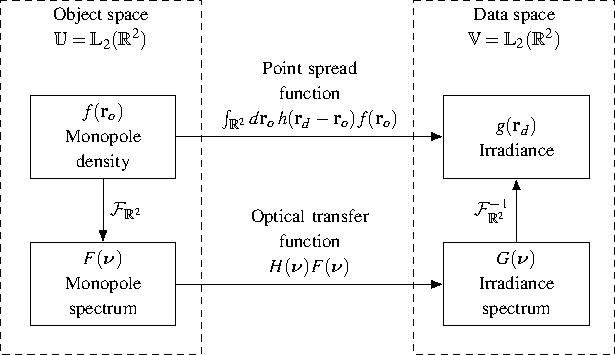
\includegraphics[scale=1.0]{../figures/monopole-block/monopole-block.pdf}
  \caption{The mapping between the object and data space of a monopole
    fluorescence microscope can be computed in two different bases---a delta
    function basis and a complex exponential basis. The change of basis can be
    computed with a two-dimensional Fourier transform denoted
    $\mathcal{F}_{\mbb{R}^2}$.}
     \label{fig:monopole-block}      
\end{figure}

The mapping between the object and the data in a linear shift-invariant imaging
system takes a particularly simple form in a complex exponential (i.e. Fourier)
basis. If we apply the Fourier convolution theorem to Eq. \eqref{eq:lsi} we find
that
\begin{align}
  G(\bv) = H(\bv)F(\bv),\label{eq:freq}
\end{align}
where we define the \textit{scaled irradiance spectrum} as
\begin{align}
  G(\bv) = \int_{\mbb{R}^2}d\mb{r}\, g(\mb{r})\, \text{exp}(-2\pi i\mb{r}\cdot\bv),
\end{align}
the \textit{monopole transfer function} as
\begin{align}
  H(\bv) = \int_{\mbb{R}^2}d\mb{r}\, h(\mb{r})\, \text{exp}(-2\pi i\mb{r}\cdot\bv),\label{eq:otf}
\end{align}
and the \textit{monopole spectrum} as
\begin{align}
    F(\bv) = \int_{\mbb{R}^2}d\mb{r}\, f(\mb{r})\, \text{exp}(-2\pi i\mb{r}\cdot\bv).
\end{align}
The monopole point spread function is normalized and real, so we know that the
monopole transfer function is normalized, $H(0) = 1$, and conjugate symmetric,
$H(-\bv) = H^*(\bv)$, where $z^*$ denotes the complex conjugate of $z$.

Notice that Eqs. \eqref{eq:lsi} and \eqref{eq:freq} are expressions of the same
mapping between object and data space in different bases. Figure
\ref{fig:monopole-block} summarizes the relationship between object and data
space in both bases.

We have been careful to use the term \textit{monopole transfer function} instead
of the commonly-used term \textit{optical transfer function}. We reserve the
term \textit{optical transfer function} for optical systems---the optical
transfer function maps between an input irradiance spectrum and an output
irradiance spectrum in an optical system. We can use optical transfer functions
to model the propagation of light through a microscope, but ultimately we are
always interested in the object, not the light emitted by the object. We will
find the distinction between the optical transfer function and the object
transfer function to be especially valuable when we consider dipoles later in
this section.

\subsubsection{Monopole coherent transfer functions}
Although the Fourier transform can be used to calculate the monopole transfer
function directly from the monopole point spread function, there is a well-known
alternative that exploits coherent transfer functions. The key idea is that the
monopole point spread function can always be written as the absolute square of a
scalar-valued \textit{monopole coherent spread function}, $c(\rd - \ro)$,
defined by
\begin{align}
  |c(\rd - \ro)|^2 = h(\rd - \ro). \label{eq:absquarescalar}
\end{align}
Physically, the monopole coherent spread function corresponds to the
scalar-valued field on the detector with appropriate scaling.

We can plug Eq. \eqref{eq:absquarescalar} into Eq. \eqref{eq:otf} and use the
autocorrelation theorem to rewrite the monopole transfer function as
\begin{align}
  H(\bv) = \int_{\mbb{R}^2}d\taup\, C(\taup)C^*(\taup - \bv), 
\end{align}
where we have introduced the
\textit{monopole coherent transfer function} as the two-dimensional Fourier
transform of the monopole coherent spread function:
\begin{align}
  C(\taup) = \int_{\mbb{R}^2}d\mb{r}\, c(\mb{r})\,\text{exp}[-2\pi i\mb{r}\cdot\taup].
\end{align}
Physically, the monopole coherent transfer function corresponds to the
scalar-valued field in a Fourier plane of the detector with appropriate scaling.

The coherent transfer function provides a valuable shortcut for analyzing
microscopes since it is often straightforward to calculate the field in a
Fourier plane of the detector. A typical approach for calculating the transfer
functions is to (1) calculate the field in a Fourier plane of the detector, (2)
scale the field to find the monopole coherent transfer function, then (3) use
the relationships in Fig. \ref{fig:monopole-transfer-functions} to calculate
the other transfer functions.

\begin{figure}
  \centering
  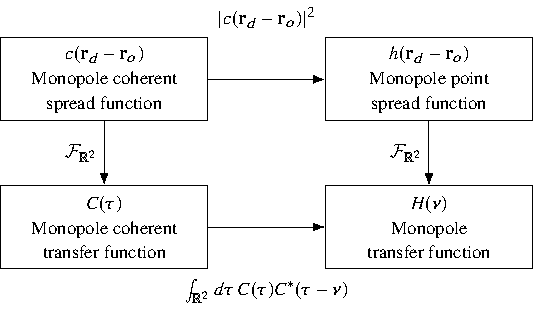
\includegraphics[scale=1.0]{../figures/monopole-transfer-functions/monopole-transfer-functions.pdf}
  \caption{The monopole transfer functions are related by a
    two-dimensional Fourier transform (right column). The coherent monopole
    transfer functions (left column) can be used to simplify the calculation of
    the remaining transfer functions.}
   \label{fig:monopole-transfer-functions}
 \end{figure}

\subsection{Dipole imaging in different bases}\label{sec:dipole}
Now we consider a microscope imaging a field of in-focus dipoles by recording
the irradiance on a two-dimensional detector. A function that assigns a real
number to each point on a plane is not sufficient to specify a field of dipoles
because the dipoles can have different orientations. To represent the object we
need to extend object space to
$\mbb{U} = \mbb{L}_2(\mbb{R}^2\times\mbb{S}^2)$---the set of square-integrable
functions on the product space of a plane and a two-dimensional sphere (the
usual sphere embedded in $\mbb{R}^3$). To visualize functions in object space we
imagine a sphere at every point on a plane with a scalar value assigned to every
point on each sphere.

In a delta function basis the object can be represented by a function
$f(\ro, \so)$ called the \textit{dipole density}---the number of dipoles per
unit area and per unit solid angle at position $\ro{}$ and oriented along
$\so{}$. Similar to the monopole case, we model the mapping between the object
and the irradiance in a delta function basis as an integral transform
\begin{align}
  g'(\rd') = \int_{\mbb{S}^2}d\so\int_{\mbb{R}^2}d\ro\, h'(\rd', \ro, \so)f(\ro, \so),
\end{align}
where $h'(\rd', \ro, \so)$ is the irradiance at position $\rd'$ created by a
point source at $\ro$ with orientation $\so$. Notice that we have considered all
possible orientations $\so$ and integrated over the sphere $\mbb{S}^2$. The
dipole density is always symmetric under angular inversion,
$f(\ro, \so) = f(\ro,-\so)$, so we could have chosen to integrate over a
hemisphere and adjusted the definition the dipole density by a factor of two.
For convenience we will continue to integrate over the complete sphere. We note
that all functions in this work with $\so$ as an independent variable are
symmetric under angular inversion, $\so \rightarrow -\so$.

If the optical system is aplanatic, we can write the
integral transform as
\begin{align}
  g'(\rd') = \int_{\mbb{S}^2}d\so\int_{\mbb{R}^2}d\ro\, h'(\rd' - m\ro, \so)f(\ro, \so). 
\end{align}

We define the same demagnified detector coordinate $\rd = \rd'/m$ and a new
normalization factor that corresponds to the total power incident on the
detector due to a spatial point source with an angularly uniform distribution of
dipoles
$P_\text{dip} = \int_{\mbb{S}^2}d\so\int_{\mbb{R}^2}d\mb{r}\, h'(m\mb{r},
\so)$. We use these scaling factors to define the
\textit{dipole point spread function} as
\begin{align}
  h(\rd - \ro, \so) = \frac{h'(m[\rd - \ro], \so)}{P_\text{dip}}, 
\end{align}
and the \textit{scaled irradiance} as 
\begin{align}
  g(\rd) = \frac{g'(m\rd)}{P_\text{dip}}. 
\end{align}
With these definitions we can express the mapping between the object and the
data as
\begin{align}
g(\rd{}) = \int_{\mbb{S}^2}d\so{}\int_{\mbb{R}^2}d\ro{}\, h(\rd{} -\ro{}, \so{})f(\ro, \so). \label{eq:odpsf}
\end{align}
Equation \eqref{eq:odpsf} is a key result because it represents the mapping
between object space and data space in a delta function basis. The integrals in
Eq. \eqref{eq:odpsf} would be extremely expensive to compute for an arbitrary
object, but the integrals simplify to an efficient sum if the object is
spatially and angularly sparse. In other words, Eq. \eqref{eq:odpsf} is ideal for
simulating and analyzing single fluorophores that are rigidly attached to an
oriented structure.

Similar to the monopole case, we have chosen to normalize the dipole point
spread function so that
\begin{align}
  \int_{\mbb{S}^2}d\so\int_{\mbb{R}^2}d\mb{r}\, h(\mb{r}, \so) = 1. 
\end{align}
The dipole point spread function is a measurable quantity, so it is real
and positive.

\subsubsection{Dipole spatial transfer function}
We can make our first change of basis by applying the Fourier-convolution
theorem to Eq. \eqref{eq:odpsf}, which yields
\begin{align}
G(\bv) = \int_{\mbb{S}^2}d\so\, H(\bv, \so)F(\bv, \so) \label{eq:odotf},
\end{align}
where we define the \textit{dipole spatial transfer function} as
  \begin{align}
  H(\bv, \so) &= \int_{\mbb{R}^2}d\mb{r}\, h(\mb{r}, \so)\, \text{exp}(-2\pi i\mb{r}\cdot\bv),\label{eq:dstf}
  \end{align}
  and the \textit{dipole spatial spectrum} as
  \begin{align}
  F(\bv, \so) &= \int_{\mbb{R}^2}d\mb{r}\, f(\mb{r}, \so)\, \text{exp}(-2\pi i\mb{r}\cdot\bv). 
  \end{align}
  Since the dipole point spread function is normalized and real, we know that
  the dipole spatial transfer function is normalized,
  $\int_{\mbb{S}^2}d\mh{s}\, H(0, \so) = 1$, and conjugate symmetric,
  $H(-\bv, \so) = H^*(\bv, \so)$.
  
  This basis is ideal for simulating and analyzing objects that are angularly
  sparse and spatially dense; e.g. rod-like structures that contain fluorophores
  in a fixed orientation, or rotationally fixed fluorophores that are undergoing
  spatial diffusion.

  \begin{figure}
  \hspace{-5em}
  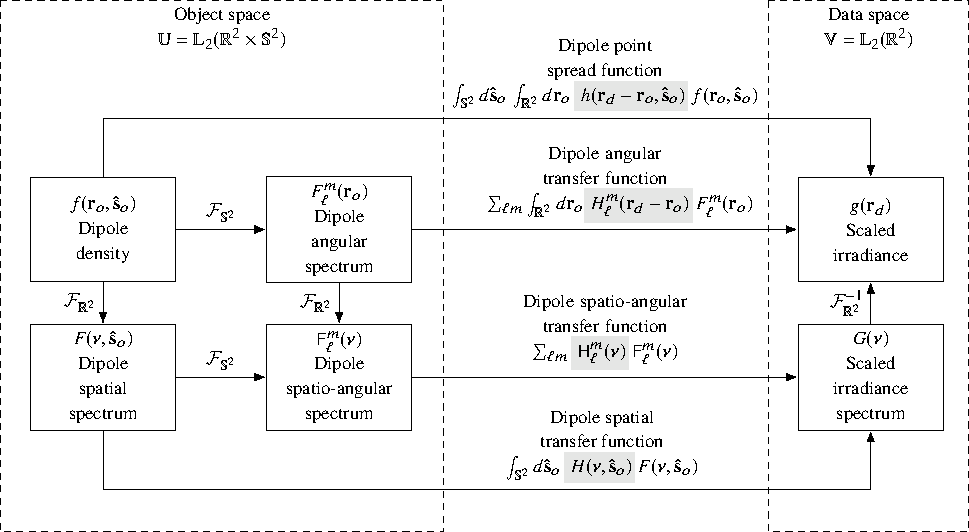
\includegraphics[scale=1.0]{../figures/dipole-block/dipole-block.pdf}
  \caption{The mapping between the object space and data space of a dipole
    imaging system can be computed in four different bases---a delta function
    basis, a complex-exponential/angular-delta basis, a
    spatial-delta/spherical-harmonic basis, and a
    complex-exponential/spherical-harmonic basis. The changes of basis can be
    computed with the two-dimensional Fourier transform denoted
    $\mathcal{F}_{\mbb{R}^2}$, and the spherical Fourier transform denoted
    $\mathcal{F}_{\mbb{S}^2}$.}
   \label{fig:dipole-block}      
    \end{figure}

\subsubsection{Dipole angular transfer function}
The spherical harmonics are another set of convenient basis functions that play
the same role as complex exponentials in spatial transfer functions---see
Appendix \ref{sec:sph} for an introduction to the spherical harmonics. We can
change basis from spherical delta functions to spherical harmonics by applying
the generalized Plancherel theorem for spherical functions
\begin{align}
  \ints{2}d\mh{s}\, p(\mh{s})q^*(\mh{s}) = \lmsum P_\ell^m Q_\ell^{m*}, \label{eq:plan}
\end{align}
where $p(\mh{s})$ and $q(\mh{s})$ are arbitrary functions on the sphere,
$P_\ell^m$ and $Q_\ell^m$ are their spherical Fourier transforms defined by
\begin{align}
  P_\ell^m = \int_{\mbb{S}^2}d\mh{s}\, p(\mh{s})Y_\ell^{m*}(\mh{s}),
\end{align}
and $Y_{\ell}^m(\mh{s})$ are the spherical harmonic functions defined in
Appendix \ref{sec:sph}. Equation \eqref{eq:plan} expresses the fact that scalar
products are invariant under a change of basis \cite[Eq.~3.78]{barrett2004}.
The left-hand side of Eq. \eqref{eq:plan} is the scalar product of
$\mbb{L}_2(\mbb{S}^2)$ functions in a delta function basis and the right-hand
side is the scalar product of $\mbb{L}_2(\mbb{S}^2)$ functions in a spherical
harmonic function basis. Applying Eq. \eqref{eq:plan} to Eq. \eqref{eq:odpsf} yields
\begin{align}
  g(\rd) = \lmsum \int_{\mbb{R}^2}d\ro\, H_\ell^m(\rd - \ro)F_\ell^m(\ro), \label{eq:atf-form}
\end{align}
where we have defined the \textit{dipole angular transfer function} as
\begin{align}
  H_\ell^m(\rd - \ro) = \int_{\mbb{S}^2}d\so\, h(\rd - \ro, \so)Y_{\ell}^{m*}(\so),\label{eq:atf-prep} 
\end{align}
and the \textit{dipole angular spectrum} as
\begin{align}
  F_\ell^m(\ro) = \int_{\mbb{S}^2}d\so\, f(\ro, \so)Y_{\ell}^{m*}(\so).
\end{align}
Since the dipole point spread function is normalized and real, we know
that the dipole angular transfer function is normalized,
$\int_{\mbb{R}^2}d\mb{r}\, H_0^0(\mb{r}) = 1$, and conjugate symmetric,
$H_\ell^{-m}(\mb{r}) = (-1)^mH_\ell^{m*}(\mb{r})$.

This basis is well suited for simulating and analyzing objects that are
spatially sparse and angularly dense; e.g. single fluorophores that are
undergoing angular diffusion, or many fluorophores that are within a resolvable
volume with varying orientations.

\subsubsection{Spatio-angular dipole transfer function}
We can arrive at our final basis in two ways: by applying the generalized
Plancherel theorem for spherical functions to Eq. \eqref{eq:odotf} or by applying
the Fourier convolution theorem to Eq. \eqref{eq:atf-form}. We follow the
first path and find that
\begin{align}
G(\bv) = \lmsum \msf{H}_\ell^m(\bv)\msf{F}_\ell^m(\bv) \label{eq:saft},
\end{align}
where we have defined the \textit{dipole spatio-angular transfer function} as
  \begin{align}
  \msf{H}_\ell^m(\bv) &= \int_{\mbb{S}^2}d\so\, H(\bv, \so)Y_\ell^{m*}(\so),
  \end{align}
  and the \textit{dipole spatio-angular spectrum} as
  \begin{align}
  \msf{F}_\ell^m(\bv) &= \int_{\mbb{S}^2}d\so\, F(\bv, \so)Y_\ell^{m*}(\so).
  \end{align}
  Since the dipole point spread function is normalized and real, we know
  that the dipole spatio-angular transfer function is normalized,
  $\msf{H}_0^0(0) = 1$, and conjugate symmetric,
  $\msf{H}_\ell^{-m}(-\bv) = (-1)^m\msf{H}_\ell^{m*}(\bv)$.
  
  This basis is well suited for simulating and analyzing arbitrary samples
  because it exploits the band limit of the imaging system. We will see the
  advantage explicitly in Section \ref{sec:results} when we calculate a specific
  dipole spatio-angular transfer function and see that it has spatial and
  angular band limits. We note that most single molecule imaging experiments
  are best described in this basis because of the effects of spatial and
  rotational diffusion.

  Figure \ref{fig:dipole-block} summarizes the relationships between the four
  bases that we can use to compute the image of a field of dipoles. We reiterate
  that all four bases may be useful depending on the sample.
    
\subsubsection{Dipole coherent transfer functions}
Similar to the monopole case, there is an efficient way to calculate the
transfer functions using coherent transfer functions. The dipole point spread
function can always be written as the absolute square of a vector-valued
function, $\mb{c}(\rd - \ro, \so)$, called the \textit{dipole coherent spread
  function}:
\begin{align}
  |\mb{c}(\rd - \ro, \so)|^2 = h(\rd - \ro, \so). \label{eq:absquare2}
\end{align}
Physically, the dipole coherent spread function corresponds to the vector-valued
electric field on the detector with appropriate scaling. We need a vector-valued
coherent transfer function since the polarization of the field plays a
significant role in dipole imaging, so the dipole point spread function cannot
be written as an absolute square of a scalar-valued function.

\begin{figure}
  \hspace{-2em}
  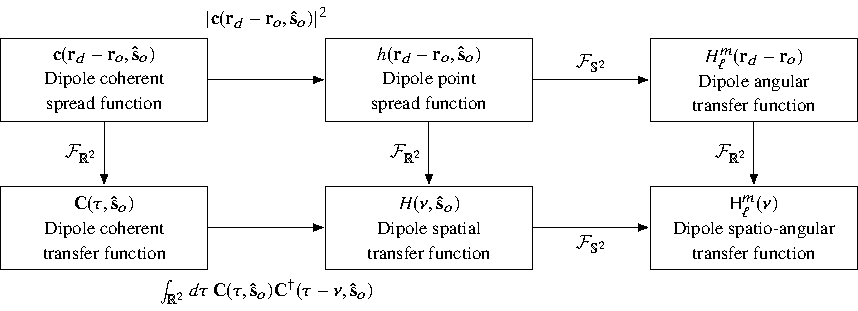
\includegraphics[scale=1.0]{../figures/transfer-functions/transfer-functions.pdf}
  \caption{There is one transfer function for each set of object-space basis
    functions, and these transfer functions are related by two-dimensional and
    spherical Fourier transforms---see center and right columns. There is an
    additional pair of coherent transfer functions that are useful for
    calculating the transfer functions---see left column.}
   \label{fig:transfer-functions}
 \end{figure}
    
We can plug Eq. \eqref{eq:absquare2} into Eq. \eqref{eq:dstf} and use the
autocorrelation theorem to rewrite the dipole spatial transfer function as
\begin{align}
  H(\bv, \so) = \int_{\mbb{R}^2}d\taup\,\mb{C}(\taup, \so)\mb{C}^\dagger(\taup - \bv, \so), 
\end{align}
where we have introduced the \textit{dipole coherent transfer function}
$\mb{C}(\taup, \so)$ as the two-dimensional Fourier transform of the dipole
coherent spread function:
\begin{align}
  \mb{C}(\taup, \so) = \int_{\mbb{R}^2}d\mb{r}\, \mb{c}(\mb{r}, \so)\,\text{exp}[-2\pi i\mb{r}\cdot\taup].
\end{align}
Physically, the dipole coherent transfer function corresponds to the
vector-valued electric field created by a dipole oriented along $\so$ in a
Fourier plane of the detector with appropriate scaling. Similar to the monopole
case, we can calculate the dipole-orientation-dependent fields in a Fourier
plane of the detector, scale appropriately to find the dipole coherent transfer
function, then use the relationships in Fig. \ref{fig:transfer-functions} to
calculate the other transfer functions. Finally, we note that the dipole
coherent transfer function is identical to what Agrawal et. al. call the
\textit{Green's tensor} \cite{agrawal2012} and Novotny and Hecht's
\textit{dyadic point spread function} multiplied by the dipole moment vector
\cite{nov2006}.

\section{Results}\label{sec:results}
In this section we begin to apply the tools we developed in the previous section
to analyze a specific fluorescence microscope. During our initial discussion we
only required the optical system to be aplanatic so that we could model it as a
shift-invariant magnifier. Now we will be more specific and consider an
aplanatic optical system in a \textit{$\mathit{4}f$ configuration} with an
arbitrary first lens (the objective lens) and a \textit{paraxial second lens}
(the tube lens) as shown in Fig. \ref{fig:schematic}. A lens can be considered
paraxial if the angle $\alpha$ between the optical axis of the lens and the
marginal ray is small enough that $\sin\alpha \approx \alpha$. As a rule of
thumb, non-paraxial effects only become significant when the numerical aperture
of a lens exceeds 0.7 \cite[ch.~6]{gu2000}, but this is only a rough
guideline. Commercial microscopes with infinity-corrected objectives can almost
always can be modeled by considering the tube lens as paraxial. 

We start by defining \textit{pupil functions} for both monopole and dipole
imaging systems, and we explicitly relate the pupil functions to the previously
defined coherent transfer functions. After establishing the link between
physical calculations and the transfer functions, we calculate the monopole and
dipole transfer functions for imaging systems with a paraxial objective, and we
demonstrate our approach by simulating simple phantoms. 

\begin{figure}[h]
 \centering
   \centering
   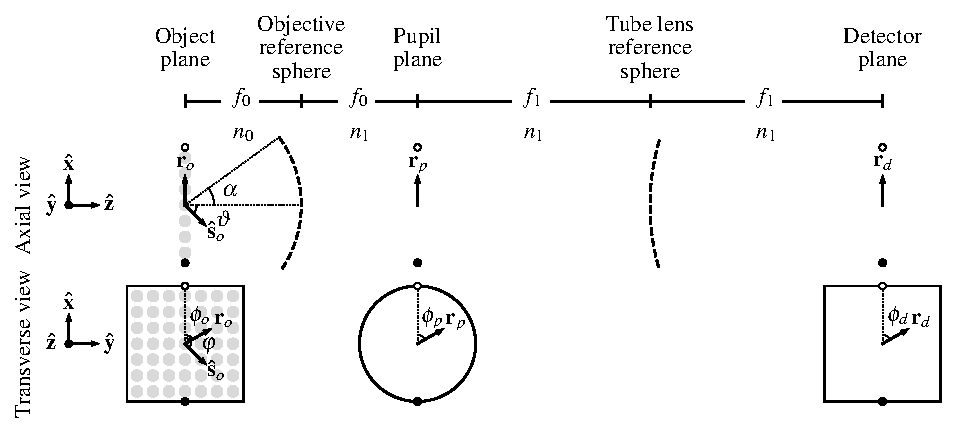
\includegraphics[width = 1.0\textwidth]{../figures/coordinates/detection-coords.pdf}
   \caption{Schematic of an aplanatic imaging system in a $4f$ geometry with a
     paraxial tube lens. We are considering an aplanatic optical system, so we
     only need to consider the image created by on-axis objects. The fluorescent
     object consists of ensembles of dipoles embedded in a medium with index of
     refraction $n_0$. An objective with focal length $f_0$ and numerical
     aperture $\text{NA} = n_o\sin\alpha$ is trained on the object. A paraxial
     tube lens with focal length $f_1$ and a detector complete the $4f$
     geometry, and all components except the object are embedded in a medium
     with index of refraction $n_1$. The object, pupil, and detector planes are
     parameterized by vectors $\ro$, $\rp$, and $\rd$ with polar coordinates
     ($r_o, \phi_o$), ($r_b, \phi_b$), and ($r_d, \phi_d$), respectively. At
     each position $\ro$ in the object there is a sphere parameterized by a unit
     vector $\so$ with spherical coordinates ($\vartheta, \varphi$). }
   \label{fig:schematic}
 \end{figure}

\subsection{Monopole pupil functions}
We define the \textit{monopole pupil function} $p(\rp)$ of the imaging system as
the field immediately following the pupil plane created by an on-axis monopole,
where $\rp$ is an unscaled two-dimensional coordinate in the pupil plane. In
this section we will relate the monopole pupil function to the transfer function
we defined in section \ref{sec:theory} by adapting the treatment in Barrett and
Myers \cite[ch.~9.7]{barrett2004}.

Since monopoles emit scalar fields, the monopole pupil function is a
scalar-valued function. The optical system is aplanatic, so we can write the
field, $U_p(\rp, \ro)$, created at a point in the pupil plane $\rp$ by a
monopole at position $\ro$ as
\begin{align}
   U_p(\rp, \ro) \propto p(\rp)\,\text{exp}\left[-2\pi i \frac{n_0}{\lambda f_0} \rp\cdot\ro \right]. \label{eq:pupil}
\end{align}
Equation \eqref{eq:pupil} is a restatement of the aplanatic condition for a $4f$
optical system---the fields in the pupil plane can be written as the pupil
function multiplied by a linear phase factor that encodes the position of the
object.

Since the second lens is paraxial, we can model the relationship between the
field in the pupil plane and the field on the detector with a scaled Fourier
transform \cite{goodman1996, axelrod2012, backer2014}:
\begin{align}
   U_d(\rd', \ro) \propto \int_{\mbb{R}^2}d\rp\, p(\rp)\,\text{exp}\left[-2\pi i \frac{n_0}{\lambda f_0} \rp\cdot\ro \right]\text{exp}\left[-2\pi i \frac{n_1}{\lambda f_1} \rp\cdot\rd' \right]. \label{eq:detectorfourier}
\end{align}

If we define $P(\taup)$ as the two-dimensional Fourier transform of the pupil function
then we can rewrite Eq. \eqref{eq:detectorfourier} as
\begin{align}
  U_d(\rd', \ro) \propto P\left(\frac{n_0}{\lambda f_0}\ro + \frac{n_1}{\lambda f_1}\rd'\right),
\end{align}
which we can simplify further by writing in terms of
$m = -\frac{f_1n_0}{f_0n_1}$:
\begin{align}
  U_d(\rd' - m\ro) \propto P\left(\frac{n_1}{\lambda f_1}[\rd' - m\ro]\right).
\end{align}
The irradiance on the detector is the absolute square of the field so
\begin{align}
  h'(\rd' - m\ro) \propto \left|P\left(\frac{n_1}{\lambda f_1}[\rd' - m\ro]\right)\right|^2.
\end{align}
If we demagnify the coordinates with $\rd = \rd'/m$ and demagnify the irradiance
with $h(\rd - \ro) \propto h'(m[\rd - \ro])$, we find that the monopole point
spread function is related to the Fourier transform of the monopole pupil
function by
\begin{align}
  h(\rd - \ro) \propto \left|P\left(-\frac{n_o}{\lambda f_o}[\rd - \ro]\right)\right|^2.
\end{align}
The monopole point spread function is the absolute square of the monopole
coherent spread function so
\begin{align}
  c(\rd - \ro) \propto P\left(-\frac{n_o}{\lambda f_o}[\rd - \ro]\right).
\end{align}
Finally, the monopole coherent transfer function is the Fourier transform of the
monopole coherent spread function so
\begin{align}
  C(\taup) \propto p\left(\frac{\lambda f_o}{n_o}\taup\right). \label{eq:monopupil0}
\end{align}
Equation \eqref{eq:monopupil0} is the key result of this section---the monopole
coherent transfer function is a scaled monopole pupil function.

\subsection{Dipole pupil function}
We define the \textit{dipole pupil function} $\mb{p}(\rp, \so)$ of the imaging
system as the electric field immediately following the pupil plane created by
an on-axis dipole oriented along $\so$. Since dipoles emit vector-valued
electric fields, the dipole pupil function is a vector-valued function. Almost
all of the arguments in the previous section carry over to the dipole case.
Briefly, we can write the electric field created at a point in the pupil
$\rp$ by a dipole at $\ro$ oriented along $\so$ as
 \begin{align}
   \mb{E}(\rp, \ro, \so) \propto \mb{p}(\rp, \so)\,\text{exp}\left[-2\pi i \frac{n_0}{\lambda f_0} \rp\cdot\ro \right]. \label{eq:pupil2}
 \end{align}
 The second lens is paraxial, so we can find the field on the detector with a
 Fourier transform
 \begin{align}
   \mb{E}_d(\rd', \ro, \so) \propto \int_{\mbb{R}^2}d\rp\, \mb{p}(\rp, \so)\,\text{exp}\left[-2\pi i \frac{n_0}{\lambda f_0} \rp\cdot\ro \right]\text{exp}\left[-2\pi i \frac{n_1}{\lambda f_1} \rp\cdot\rd' \right]. \label{eq:detectorfourier2}
\end{align}
Note that the Fourier transform of a vector field is the Fourier transform of
its scalar-valued orthogonal components, so Eq. \eqref{eq:detectorfourier2}
specifies three two-dimensional Fourier transforms. We follow the same
manipulations as the previous section and find that the dipole coherent transfer
function is a scaled dipole pupil function
\begin{align}
  \mb{C}(\taup, \so) \propto \mb{p}\left(\frac{\lambda f_o}{n_o}\taup, \so\right). \label{eq:monopupildip}
\end{align}

We have restricted our analysis to paraxial tube lenses, but non-paraxial tube
lenses (or a non-infinity-corrected objective) can be modeled with vector-valued
three-dimensional pupil functions \cite{sheppard1994, gu2000, arnison2002,
  foreman2011-2}.

\subsection{Special functions}
We adopt and generalize Bracewell's notation \cite{bracewell2004} for several
special functions which will simplify our calculations. First, we define a
\textit{rectangle function} as
\begin{align}
  \Pi(x) = 
  \begin{cases}
    1\quad \text{if}\quad |x| < \frac{1}{2},\\
    0\quad \text{else}.
  \end{cases}
\end{align}
We also define the \textit{$n^{th}$-order jinc function} as
\begin{align}
  \text{jinc}_n(r) = \frac{J_{n+1}(\pi r)}{2r},
\end{align}
where $J_{n+1}(r)$ is the $(n+1)^{th}$-order Bessel function of the first kind.

Although the rectangle and jinc functions are defined in one dimension, we will
usually apply them in two dimensions. In Appendix \ref{sec:special} we derive
the following two-dimensional Fourier transform relationships between the jinc
functions and the weighted rectangle functions
\begin{align}
  i^{n}\left\{\substack{
  \text{exp}(in\phi_r)\\
    \cos(n\phi_r)\\
    \sin(n\phi_r)
  }\right\}\text{jinc}_n(r) &\stackrel{\mathcal{F}_{\mbb{R}^2}}{\longrightarrow} (2\nu)^{n}\left\{\substack{
    \text{exp}(in\phi_{\nu})\\
    \cos(n\phi_{\nu})\\
    \sin(n\phi_{\nu})
  }\right\}\Pi(\nu), \label{eq:jincrect2}
  \end{align}
  where the entries inside the curly braces are to be taken one at a time and
  $\{r, \phi_r\}/\{\nu, \phi_\nu\}$ are conjugate sets of polar coordinates.
  
Finally, we define the \textit{$n^{th}$-order chat function} as the
two-dimensional Fourier transform of the squared $n^{th}$-order jinc function
\begin{align}
  \text{jinc}_n^2(r) \stackrel{\mathcal{F}_{\mbb{R}^2}}{\longrightarrow} \text{chat}_n(\nu).
\end{align}

In Appendix \ref{sec:special} we show that the zeroth- and first-order chat
functions can be written in closed form as
\begin{align}
  \text{chat}_0(x) &=  \frac{1}{2}\left[\cos^{-1}|x| - |x|\sqrt{1 - x^2}\right]\Pi\left(\frac{x}{2}\right),\\
  \text{chat}_1(x) &=  \frac{1}{2}\left[\cos^{-1}|x| - |x|(3-2x^2)\sqrt{1 - x^2}\right]\Pi\left(\frac{x}{2}\right).  
\end{align}


\subsection{Monopole transfer functions}
Our first step towards the monopole transfer functions is to calculate the
monopole pupil function and coherent transfer function. Several works
\cite{petrov2017, backlund2018} have modeled an aplanatic fluorescence
microscope imaging monopole emitters with the scalar pupil function
\begin{align}
  p(\rp) \propto \tilde{C}\left(\frac{r_p}{f_o}\right)\Pi\left(\frac{r_p}{2f_o\sin\alpha}\right), 
\end{align}
where
\begin{align}
  \tilde{C}(x) = (1 - x^2)^{-1/4} = 1 + \frac{x^2}{4} + \frac{5x^4}{32} + \cdots. 
\end{align}
The $\tilde{C}(x)$ function models the radial dependence of the field and
ensures that power is conserved on either side of an aplanatic objective, and
the rectangle function models the aperture stop of the objective. Applying Eq.
\eqref{eq:monopupil0} and collecting constants we find that the coherent monopole
transfer function is
\begin{align}
  C(\taup) \propto \tilde{C}\left(\frac{2\text{NA}}{n_o}\frac{\tau}{\nu_c}\right)\Pi\left(\frac{\tau}{\nu_c}\right), \label{eq:coherentmonopole}
\end{align}
where $\text{NA} = n_o\sin\alpha$ and $\nu_c = 2\text{NA}/\lambda$. This
coherent transfer function models objectives with an arbitrary numerical
aperture, but for our initial analysis we restrict ourselves to the paraxial
regime. We drop second- and higher-order radial terms to find that
\begin{align}
  C(\taup) \stackrel{(p)}{\propto} \Pi\left(\frac{\tau}{\nu_c}\right), 
\end{align}
where $(p)$ indicates that we have used the paraxial approximation for the
objective lens.

We can find the monopole coherent spread function by taking the inverse Fourier
transform of the monopole coherent transfer function
\begin{align}
  c(\mb{r}) \stackrel{(p)}{\propto} \text{jinc}_0(\nu_c r).
\end{align}

The monopole point spread function is the (normalized) absolute square of the
monopole coherent spread function so
\begin{align}
  h(\mb{r}) \stackrel{(p)}{=} \frac{4}{\pi}\text{jinc}_0^2(\nu_c r),
\end{align}
which is the well-known \textit{Airy disk}.

Finally, we can calculate the monopole transfer function as the two-dimensional Fourier transform of the monopole point spread function (or the autocorrelation
of the coherent transfer function) and find that 
\begin{align}
  H(\bs{\nu}) \stackrel{(p)}{=} \frac{4}{\pi}\text{chat}_0\left(\frac{\nu}{\nu_c}\right).
\end{align}

 \subsection{Dipole transfer functions}
 To calculate the dipole transfer function we proceed similarly to the monopole
 case---we find the pupil function, scale to find the coherent dipole transfer
 function, then calculate the remaining transfer functions.
 
 Backer and Moerner \cite{backer2014} have calculated the dipole pupil function
 for a high-NA objective as
 \begin{align}
   \mb{p}(\rp, \so) \propto
   \begin{bmatrix}
     \tilde{C}_0\left(\frac{r_p}{f_o}\right) + \tilde{C}_2\left(\frac{r_p}{f_o}\right)c(2\phi_p)&\tilde{C}_2\left(\frac{r_p}{f_o}\right)s(2\phi_p)&\tilde{C}_1\left(\frac{r_p}{f_0}\right)c(\phi_p)\\
     \tilde{C}_2\left(\frac{r_p}{f_o}\right)s(2\phi_p)&\tilde{C}_0\left(\frac{r_p}{f_o}\right) - \tilde{C}_2\left(\frac{r_p}{f_o}\right)c(2\phi_p)&\tilde{C}_1\left(\frac{r_p}{f_0}\right)s(\phi_p)\\     
     0&0&0\\     
   \end{bmatrix}
   \begin{bmatrix}
     s_x\\
     s_y\\
     s_z
   \end{bmatrix}
   \Pi\left(\frac{r_p}{2f_os(\alpha)}\right),
 \end{align}
 where $c(x)$ and $s(x)$ are shorthand for $\cos(x)$ and $\sin(x)$,
 $\{s_x, s_y, s_z\}$ are the Cartesian components of $\so$ when $\mh{z}$ is
 aligned with the optical axis, and
 \begin{alignat}{4}
   \tilde{C}_0(x) &= \frac{1}{2}\left(\sqrt{1 - x^2} + 1\right)(1 - x^2)^{-1/4} &&= 1 + \frac{x^4}{32} + \frac{x^6}{32} + \cdots,\\
   \tilde{C}_1(x) &= x(1 - x^2)^{-1/4} &&= x + \frac{x^3}{4} + \frac{5x^5}{32} + \cdots,\\
   \tilde{C}_2(x) &= \frac{1}{2}\left(\sqrt{1 - x^2} - 1\right)(1 - x^2)^{-1/4} &&= -\frac{x^2}{4} - \frac{x^4}{8} - \frac{11x^6}{128} - \cdots.
 \end{alignat}
 Similar to the monopole case, the dipole pupil function conserves power and has
 a cutoff at the objective aperture, but the dipole pupil function is
 vector-valued to model the complete electric field in the pupil plane. The
 fields in the pupil plane have a negligible $\mh{z}$ component which is a
 consequence of our assumption that the tube lens is paraxial---modeling a
 non-paraxial tube lens would require a three-dimensional vector-valued pupil
 function \cite{sheppard1994, gu2000, arnison2002, foreman2011-2}. 

 Scaling the dipole pupil function using Eq. \eqref{eq:monopupildip} yields the
 dipole coherent transfer function
 \begin{equation}
   \mb{C}(\taup, \so)\hspace{-0.2em}\propto\hspace{-0.2em}
   \begin{bmatrix}
     \tilde{C}_0\left(\frac{\lambda r_p\tau}{n_0}\right)\!+\!\tilde{C}_2\left(\frac{\lambda r_p\tau}{n_0}\right)c(2\phi_{\tau})&\tilde{C}_2\left(\frac{\lambda r_p\tau}{n_0}\right)s(2\phi_{\tau})&\tilde{C}_1\left(\frac{\lambda r_p\tau}{n_0}\right)c(\phi_{\tau})\\
     \tilde{C}_2\left(\frac{\lambda r_p\tau}{n_0}\right)s(2\phi_{\tau})&\tilde{C}_0\left(\frac{\lambda r_p\tau}{n_0}\right)\!-\!\tilde{C}_2\left(\frac{\lambda r_p\tau}{n_0}\right)c(2\phi_{\tau})&\tilde{C}_1\left(\frac{\lambda r_p\tau}{n_0}\right)s(\phi_{\tau})\\     
     0&0&0\\     
   \end{bmatrix}
   \begin{bmatrix}
     s_x\\
     s_y\\
     s_z
   \end{bmatrix}
   \Pi\left(\frac{\tau}{\nu_c}\right). 
 \end{equation}
 We restrict our analysis to the paraxial regime by dropping second- and
 higher-order radial terms to find that
 \begin{align}
   \mb{C}(\taup, \so) \stackrel{(p)}{\propto}
   \begin{bmatrix}
     1&0&\frac{\text{2NA}}{n_o}\frac{\tau}{\nu_c}\cos\phi_{\tau}\\
     0&1&\frac{\text{2NA}}{n_o}\frac{\tau}{\nu_c}\sin\phi_{\tau}\\
     0&0&0\\     
   \end{bmatrix}
   \begin{bmatrix}
     s_x\\
     s_y\\
     s_z
   \end{bmatrix}
   \Pi\left(\frac{\tau}{\nu_c}\right). \label{eq:coherentdip}
 \end{align}
 Under the paraxial approximation the transverse components of the dipole
 \{$s_x, s_y$\} create purely transverse fields in the pupil plane and the axial
 component of the dipole \{$s_z$\} creates purely radial fields in the pupil
 plane. The paraxial approximation may seem crude compared to Backer and
 Moerner's numerical results, but the approximation will allow us to calculate
 the transfer functions in closed form so that we can build an intuition for the
 limits of the microscope. We also note that many existing works in ensemble
 polarized fluorescence microscopy make stronger approximations than ours. For
 example, Fourkas only considers the total irradiance in the pupil plane while
 ignoring the propagation of fields to the detector \cite{fourkas2001}.

 The dipole coherent spread function is the inverse Fourier transform of the
 dipole coherent transfer function. Applying Eq. \eqref{eq:jincrect2} in reverse
 yields
  \begin{align}
   \mb{c}(\mb{r}, \so) \stackrel{(p)}{\propto}
   \begin{bmatrix}
     \text{jinc}_0(\nu_c r)&0&\frac{\text{NA}}{n_o}i\cos\phi\,\text{jinc}_1(\nu_c r)\\
     0&\text{jinc}_0(\nu_c r)&\frac{\text{NA}}{n_o}i\sin\phi\,\text{jinc}_1(\nu_c r)\\
     0&0&0\\     
   \end{bmatrix}
   \begin{bmatrix}
     s_x\\
     s_y\\
     s_z
   \end{bmatrix}.
  \end{align}
  Notice that the radial component of the dipole coherent spread function has a
  $\pi/2$ phase shift relative to the transverse component. This phase factor
  arises because the Fourier transform of a real and odd function is purely
  imaginary.
  
  \subsubsection{Paraxial dipole point spread function}
  The dipole point spread function is the (normalized) absolute square of the
coherent dipole spread function
\begin{align}
  h(\mb{r}, \so) \propto \mb{c}(\mb{r}, \so)\mb{c}^\dagger(\mb{r}, \so). 
\end{align}
Plugging in the paraxial dipole coherent spread function and normalizing yields
\begin{align}
  h(\mb{r}, \so) \stackrel{(p)}{=} N\left[\text{jinc}_0^2(\nu_c r)\sin^2\vartheta + \left(\frac{\text{NA}}{n_o}\right)^2\text{jinc}_1^2(\nu_c r)\cos^2\vartheta\right],\label{eq:paradpsf}
\end{align}
where $\sin^2\vartheta = s_x^2 + s_y^2$, $\cos^2\vartheta = s_z^2$, and the normalization
factor is
\begin{align}
  N = 6\nu_c^2\pi^{-3/2}\left[2 + \left(\frac{\text{NA}}{n_o}\right)^2\right]^{-1}.
\end{align}

As discussed above, the transverse and radial fields are out of phase on the
detector, so the total irradiance is the sum of the contributions from the
transverse and radial components. In Fig. \ref{fig:hdet} we plot the dipole
point spread function for several dipole orientations and numerical apertures,
and in Fig. \ref{fig:microscopefig} we compare the monopole point spread
function to the dipole point spread function. The paraxial monopole and dipole
models are only equivalent when the sample consists of transverse dipoles, which
is clear if we notice that Eq. \eqref{eq:paradpsf} reduces to an Airy disk when
$\vartheta = \pi/2$---see Novotny and Hecht for a similar observation
\cite[ch.~4]{nov2006}.

\begin{figure}[h]
 \centering
   \centering
   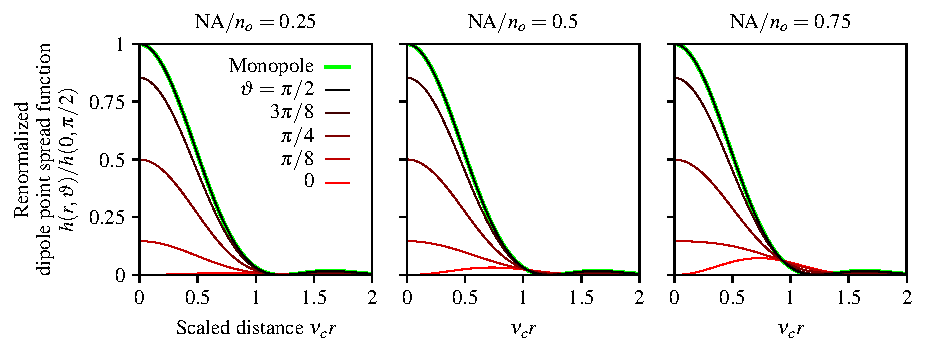
\includegraphics[scale=0.8]{../figures/paratfs/dpsf.pdf}
   \caption{Renormalized paraxial dipole point spread function as a function of
     the scaled radial coordinate $\nu_c r$, the dipole inclination angle
     $\vartheta$, and $\text{NA}/n_o$. For small numerical apertures (left) the
     irradiance pattern created by axial dipoles (\textcolor{red}{\textbf{red}})
     is small compared to transverse dipoles (\textbf{black}), but the relative
     contribution of axial dipoles increases with the numerical aperture (see
     \textcolor{red}{\textbf{red}} lines from left to right). Additionally, we
     plot the monopole point spread function (\textcolor{green}{\textbf{green}})
     and observe that the paraxial monopole and dipole models are identical for
     transverse dipoles (the \textcolor{green}{\textbf{green}} and
     \textbf{black} lines are coincident).}
   \label{fig:hdet}
 \end{figure}
 
\begin{figure}[h]
 \centering
   \centering
   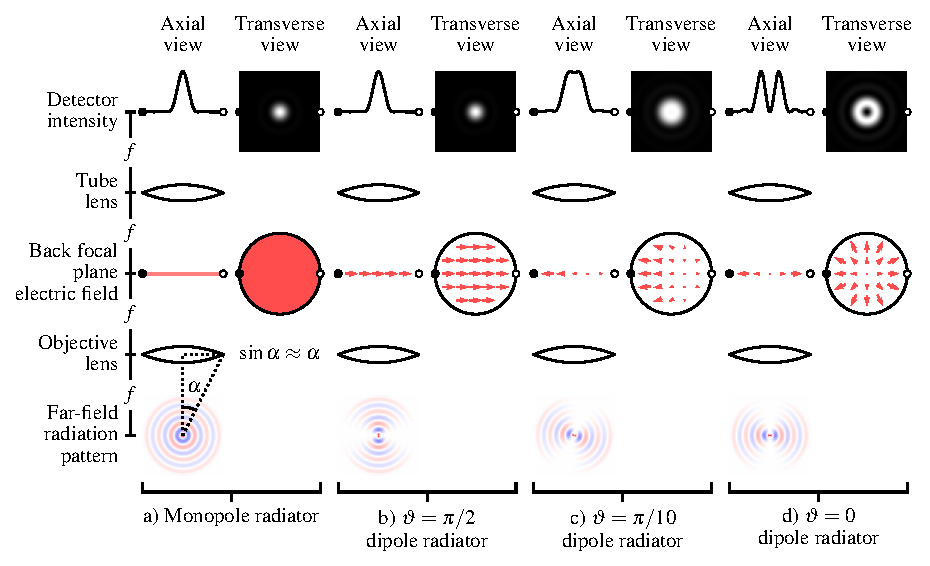
\includegraphics[scale=0.8]{../figures/microscope/microscope.pdf}
   \caption{Comparison of paraxial models for monopole radiators a) and dipole
     radiators b)--d). a) Monopole radiators fill the pupil plane with a uniform
     scalar field which gives rise to an Airy disk on the detector. b) A
     transverse dipole radiator also creates an Airy disk, but the pupil plane
     is filled with a uniform vector field. c) An axial dipole radiator creates
     a radial electric field pattern in the back focal plane that creates a
     $\text{jinc}_1^2(r)$ pattern on the detector. d) Dipoles that are not
     transverse or axial still create radially symmetric irradiance patterns
     under the paraxial approximation. Fields from transverse dipoles are real
     and even while fields from axial dipoles are real and odd, which causes a
     relative $\pi/2$ phase shift for the fields on the detector. This phase
     shift means that the fields from transverse and axial components of the
     dipole do not interfere, which causes radially symmetric irradiance
     patterns.}
   \label{fig:microscopefig}
 \end{figure}

 To demonstrate the paraxial dipole point spread function we simulate a set of
 equally spaced dipoles with varying orientation:
 \begin{align}
   f_{(ph1)}(r_x, r_y, \vartheta, \varphi) = \sum_{j=0}^3 \sum_{k=0}^3 \delta\left(r_x - j\right)\, \delta\left(r_y - k\right)\, \delta\left(\cos\vartheta - \cos\vartheta_j\right)\, \delta\left(\varphi - \varphi_k\right),\label{eq:phantom1}
 \end{align}
 where $\vartheta_j = j\frac{\pi}{6}$, $\varphi_k = k\frac{\pi}{4}$, the
 subscript $(ph1)$ indicates that this is the first phantom, and the spatial
 coordinates are expressed in $\mu$m. To find the irradiance pattern created by
 the phantom we plug Eq. \eqref{eq:phantom1} into Eq. \eqref{eq:odpsf} and use
 the sifting property to find that
 \begin{align}
   g_{(ph1)}(r_x, r_y) = \sum_{j=0}^3 \sum_{k=0}^3 h\left(\sqrt{\left(r_x - j\right)^2 + \left(r_y - k\right)^2}, \vartheta_j\right).\label{eq:phantom1irr}
 \end{align}
 In Fig. \ref{fig:ph1} we plot the phantom and scaled irradiance for an imaging
 system with $\text{NA} = 0.75$, $\lambda = 500\,\text{nm}$, and $n_o = 1.33$.
 We sample and plot the scaled irradiance at $20\times$ the Nyquist rate,
 $\Delta x = 1/[20(2\nu_c)]$, so the irradiance patterns are free of aliasing.
 The output demonstrates that the irradiance pattern depends on the dipole
 inclination, but not its azimuth.

 \begin{figure}[h]
 \centering
   \centering
   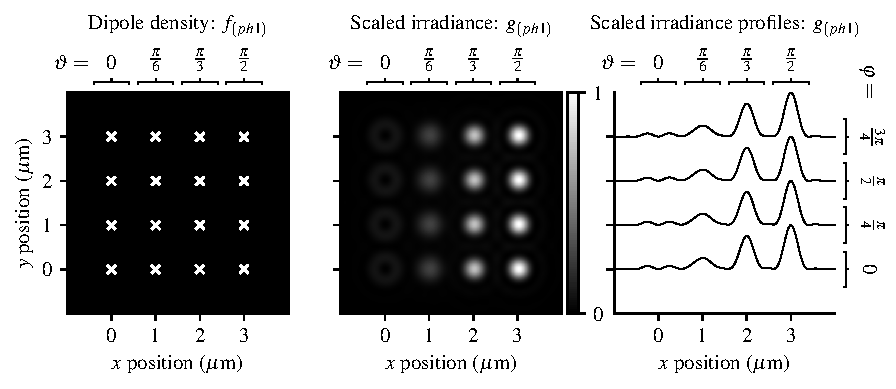
\includegraphics[scale=0.8]{../figures/paratfs/ph1.pdf}
   \caption{\textbf{Left:} A spatially and angularly sparse phantom---uniformly
     spaced single dipoles with varying orientations (increasing $\vartheta$
     from left to right and increasing $\varphi$ from bottom to top). White
     crosses mark the positions of the dipoles. \textbf{Center:} Scaled
     irradiance for an imaging system with $\text{NA} = 0.75$,
     $\lambda = 500\,\text{nm}$, and $n_o = 1.33$ sampled at $20\times$ the
     Nyquist rate. \textbf{Right:} $x$ profiles through the scaled irradiance.
     The response is independent of the azimuth angle and strongly dependent on
     the inclination angle.}
   \label{fig:ph1}
 \end{figure}

\subsubsection{Paraxial dipole spatial transfer function}\label{sec:trans}
The dipole spatial transfer function is the spatial Fourier transform of
the dipole point spread function (or the complex autocorrelation of the dipole
coherent transfer function). Applying the Fourier transform to Eq.
\eqref{eq:paradpsf} we find that
  \begin{align}
    H(\bs{\nu}, \vartheta) \stackrel{(p)}{=} \frac{N}{\nu_c^2}\left[\text{chat}_0\left(\frac{\nu}{\nu_c}\right)\sin^2\vartheta + \left(\frac{\text{NA}}{n_o}\right)^2 \text{chat}_1\left(\frac{\nu}{\nu_c}\right)\cos^2\vartheta\right].
  \end{align}
In Fig. \ref{fig:odotf} we plot the dipole spatial transfer function for
several dipole orientations and numerical apertures. We find that the dipole
spatial transfer function is negative for axial dipoles at high spatial
frequencies, especially for larger numerical apertures. The negative dipole
spatial transfer corresponds to a contrast inversion for high-frequency
patterns of axial dipoles because the irradiance minimum corresponds to the
position of the dipole.

\begin{figure}[h]
 % \captionsetup{width=1.0\linewidth}
 \centering
   \centering
   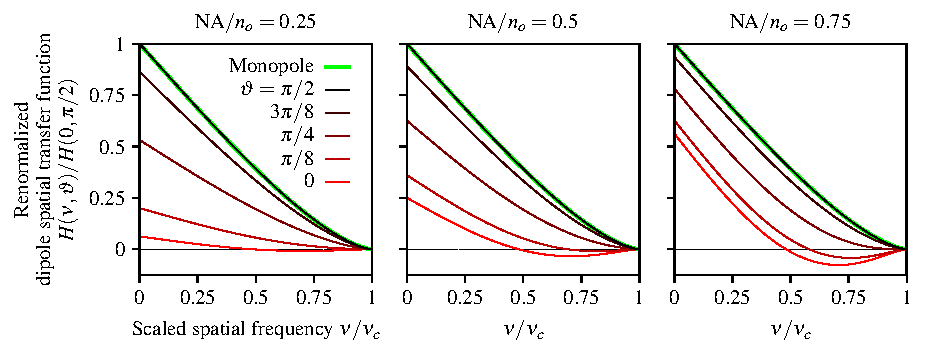
\includegraphics[scale=0.8]{../figures/paratfs/sdtf.pdf}
   \caption{Dipole spatial transfer function as a function of the scaled spatial
     frequency $\nu/\nu_c$, the dipole inclination angle $\vartheta$, and
     $\text{NA}/n_o$. For small numerical apertures (left) the dipole spatial
     transfer function for axial dipoles (\textcolor{red}{\textbf{red}}) is
     small compared to transverse dipoles (\textbf{black}), but the relative
     contribution of axial dipoles increases with the numerical aperture (see
     \textcolor{red}{\textbf{red}} lines from left to right). The spatial dipole
     transfer function of axial dipoles is negative at high spatial frequencies
     because the central minimum of the axial dipole point spread function
     corresponds to the position of the dipole. Equivalently, a
     high-spatial-frequency pattern of axial dipoles will generate an irradiance
     pattern where the minimum irradiance corresponds to the peak of the axial
     dipole density. Additionally, we plot the monopole transfer function
     (\textcolor{green}{\textbf{green}}) and observe that the paraxial monopole
     and dipole models are identical for transverse dipoles (the
     \textcolor{green}{\textbf{green}} and \textbf{black} lines are
     coincident).}
   \label{fig:odotf}
 \end{figure}

 To demonstrate the dipole spatial transfer function we simulate a set of
 equally spaced disks with varying diameter containing fluorophores with varying
 orientation
 \begin{align}
   f_{(ph2)}(r_x, r_y, \vartheta) = \sum_{j=0}^3 \sum_{k=0}^3 \frac{1}{D_k^2}\Pi\left(\frac{1}{D_k}\sqrt{\left(r_x - j\right)^2 + \left(r_y - k\right)^2}\right) \delta\left(\cos\vartheta - \cos\vartheta_j\right)\,\label{eq:phantom2}
 \end{align}
 where $D_k = 0.15(1+k)\, \mu$m and $\vartheta_j = j\frac{\pi }{6}$. Notice that
 we have scaled the disks so that the total number of fluorophores in each disk
 is constant. Also notice that the disk can model a spatial distribution of many
 fluorophores or a single molecule undergoing spatial diffusion within a well.  

 We can calculate the irradiance pattern by taking the spatial Fourier transform
 for each orientation in the phantom, filtering the result with the dipole
 spatial transfer function, integrating over the orientations, then taking the
 inverse spatial Fourier transform. Since our phantom is angularly sparse, the
 integral becomes a sum and we find that
 \begin{align}
   g_{(ph2)}(r_x, r_y) = \mc{F}^{-1}_{\mbb{R}^2}\left\{\sum_{j}H(\nu, \vartheta_j)\mc{F}_{\mbb{R}^2}\left\{f_{(ph2)}(r_x, r_y, \vartheta_j)\right\}\right\}.
 \end{align}

 In Fig. \ref{fig:ph2} we plot the phantom and scaled irradiance with the same
 imaging parameters as the previous section. The small disks create irradiance
 patterns that are similar to the point sources in the previous section, while
 larger disks create increasingly uniform irradiance patterns that hide the
 orientation of the fluorophores.
  
  \begin{figure}[h]
 % \captionsetup{width=1.0\linewidth}
 \centering
   \centering
   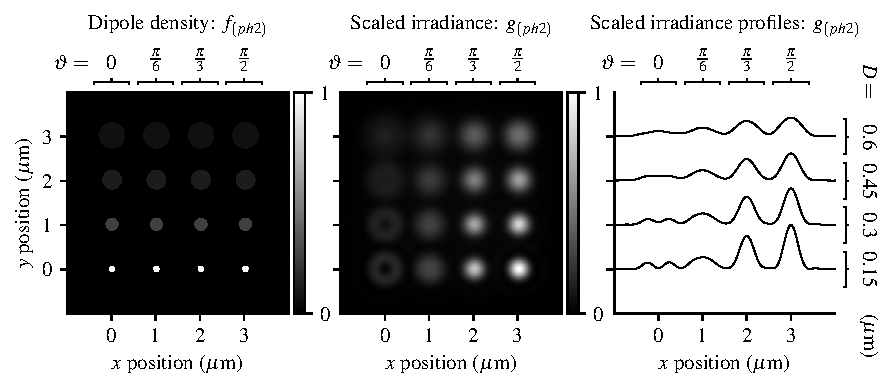
\includegraphics[scale=0.8]{../figures/paratfs/ph2.pdf}
   \caption{\textbf{Left:} A spatially dense and angularly sparse
     phantom---uniformly spaced disks with varying size (increasing $D$ from
     bottom to top) and dipole orientation (increasing $\vartheta$ from left to
     right) \textbf{Center:} Scaled irradiance for an imaging system with
     $\text{NA} = 0.75$, $\lambda = 500\,\text{nm}$, and $n_o = 1.33$ sampled at
     $20\times$ the Nyquist rate. \textbf{Right:} $x$ profiles through the
     scaled irradiance. Larger disks generate increasingly uniform irradiance
     patterns with fewer details that may indicate the orientation of
     fluorophores.}
   \label{fig:ph2}
 \end{figure}

 \subsubsection{Paraxial dipole angular transfer function}
 To calculate the angular dipole transfer function we take the spherical Fourier
 transform of the dipole point spread function
 \begin{align}
H_l^m(\mb{r}) \stackrel{}{=} \int_{\mbb{S}^2}d\so\, h(\mb{r}, \so)Y_l^{m*}(\so).
 \end{align}
 After evaluating the integrals and normalizing, the angular dipole transfer
 function is
 \begin{align}
   H_l^m(\mb{r}) \stackrel{(p)}{=} &\frac{N}{3}\left[2\text{jinc}_0^2(\nu_cr) + \left(\frac{\text{NA}}{n_o}\right)^2\text{jinc}_1^2(\nu_c r)\right]\Lambda_0\delta_{\ell0}\delta_{m0} + \nonumber\\& \frac{N}{3}\left[-2\text{jinc}_0^2(\nu_c r) + 2\left(\frac{\text{NA}}{n_o}\right)^2\text{jinc}_1^2(\nu_c r)\right]\Lambda_2\delta_{\ell2}\delta_{m0},
 \end{align}
where $\Lambda_{\ell} = \sqrt{4\pi/(2\ell + 1)}$. 

In Fig. \ref{fig:atf} we plot the dipole angular transfer function for both
spherical harmonic terms and several numerical apertures. Note that the dipole
angular transfer function can be negative because the spherical harmonics can
take negative values. The $\ell=0$ term shows that angularly uniform
distributions of dipoles create spatial irradiance patterns that are similar but
not identical to the Airy disk, while the $\ell=2$ term shows a negative pattern
because of the large contribution of the transverse negative values in the
$Y_2^0$ spherical harmonic.

\begin{figure}[h]
 \centering
   \centering
   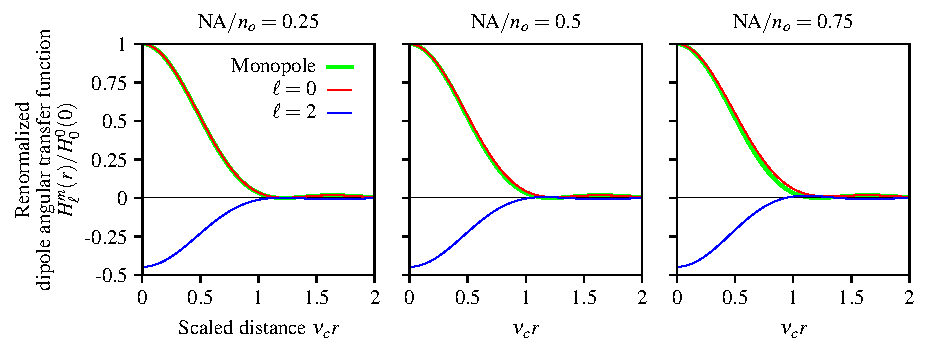
\includegraphics[scale=0.8]{../figures/paratfs/adtf.pdf}
   \caption{Paraxial dipole angular transfer function in terms of a scaled
     radial detection coordinate $\nu_c r$, the spherical harmonic degree
     $\ell$, and $\text{NA}/n_o$. Angularly uniform distributions of dipoles
     $\ell=0$ generate a spatial pattern that is similar but not identical to
     the Airy disk created by a monopole (\textcolor{green}{\textbf{green}}),
     and this discrepancy increases with the numerical aperture. $\ell=2$
     distributions have a negative response because $Y_2^0(\mh{s})$ is negative
     for transverse directions. As the numerical aperture increases, the
     relative contribution of positive axial dipoles in the $\ell=2$
     distribution increases.}
   \label{fig:atf}
 \end{figure}

 To demonstrate the dipole angular transfer function we simulate a set of
 equally spaced fluorophore distributions with varying orientation and angular
 distributions
 \begin{align}
   f_{(ph3)}(r_x, r_y, \vartheta) = \sum_{j=0}^3 \sum_{k=0}^3 \delta\left(r_x - j\right)\, \delta\left(r_y - k\right)\, f_{\text{(cone)}}\left(\vartheta, \varphi; \vartheta_j, 0, \Delta_k\right),\label{eq:phantom3}
 \end{align}
 where
 \begin{align}
   f_{\text{(cone)}}(\so; \so', \Delta) = f_{\text{(cone)}}(\vartheta, \varphi; \vartheta', \varphi', \Delta) = \frac{1}{4\pi(1 - \cos\Delta)}\Pi\left(\frac{\mh{s}\cdot\mh{s}'}{2\cos\Delta}\right)
 \end{align}
 is an angular double cone distribution with central direction $\mh{s}'$ and
 cone half-angle $\Delta$; $\vartheta_j = j\frac{\pi}{6}$; and
 $\Delta_k = k\frac{\pi}{6}$. Notice that when $\Delta = 0$ the angular double
 cone reduces to a single direction, and when $\Delta = \pi/2$ the angular
 double cone reduces to an angularly uniform distribution. Also notice that the
 double cone can model angular diffusion or the angular distribution of many
 fluorophores within a resolvable volume.
 
 Our first step towards the irradiance pattern is to calculate the dipole
 angular spectrum of the phantom. In Appendix \ref{sec:cone} we calculate the
 spherical Fourier transform of the double cone distribution
 $F^m_{\ell,\text{(cone)}}(\vartheta', \varphi'; \Delta)$ which we can use to
 express the dipole angular spectrum as
 \begin{align}
   F^{m}_{\ell,(ph3)}(r_x, r_y, \vartheta) = \sum_{j=0}^3 \sum_{k=0}^3 \delta\left(r_x - j\right)\, \delta\left(r_y - k\right)\, F^m_{\ell,\text{(cone)}}\left(\vartheta_j, 0, \Delta_k\right).\label{eq:phantom3spect}
 \end{align}

 To find the irradiance we plug the dipole angular spectrum into Eq.
 \eqref{eq:atf-form} and use the sifting property to find that
 \begin{align}
   g_{(ph3)}(r_x, r_y) = \sum_{\ell m}\sum_{j=0}^3 \sum_{k=0}^3 H_\ell^m\left(\sqrt{\left(r_x - j\right)^2 + \left(r_y - k\right)^2}\right) F^m_{\ell,\text{(cone)}}\left(\vartheta_j, 0, \Delta_k\right).\label{eq:phantom3irr}
 \end{align}

 In Fig. \ref{fig:ph3} we plot the phantom and scaled irradiance with the same
 imaging parameters as the previous sections. For small cone angles the
 irradiance patterns are similar to the point sources in the previous sections,
 while larger cone angles create increasingly uniform irradiance patterns that
 hide the angular information about the distributions.

  \begin{figure}[h]
 \centering
   \centering
   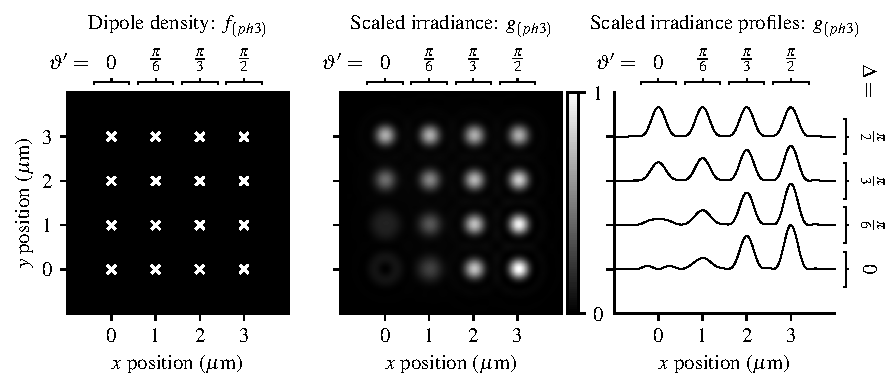
\includegraphics[scale=0.8]{../figures/paratfs/ph3.pdf}
   \caption{\textbf{Left:} A spatially sparse and angularly dense
     phantom---uniformly spaced double cone distributions of fluorophores with
     varying central direction (increasing $\vartheta'$ from left to right) and
     varying cone half-angle (increasing $\Delta$ from bottom to top).
     \textbf{Center:} Scaled irradiance for an imaging system with
     $\text{NA} = 0.75$, $\lambda = 500\,\text{nm}$, and $n_o = 1.33$ sampled at
     $20\times$ the Nyquist rate. \textbf{Right:} $x$ profiles through the
     scaled irradiance. Small cone angles have irradiance patterns that vary
     with the central direction, while larger cones angles have increasingly
     uniform irradiance patterns that hide angular information.}
   \label{fig:ph3}
 \end{figure}

 \subsubsection{Paraxial dipole spatio-angular transfer function}
 We can calculate the dipole spatio-angular transfer function by taking the
 spatial Fourier transform of the dipole angular transfer function (or the
 spherical Fourier transform of the dipole spatial transfer function) to find
 that
 \begin{align}
H_{\ell}^m(\bv) \stackrel{(p)}{=} &\frac{N}{3\nu_c^2}\left[2\text{chat}_0\left(\frac{\nu}{\nu_c}\right) + \left(\frac{\text{NA}}{n_o}\right)^2\text{chat}_1\left(\frac{\nu}{\nu_c}\right)\right]\Lambda_0\delta_{\ell0}\delta_{m0}+\nonumber\\ &\frac{N}{3\nu_c^2}\left[-2\text{chat}_0\left(\frac{\nu}{\nu_c}\right) + 2\left(\frac{\text{NA}}{n_o}\right)^2\text{chat}_1\left(\frac{\nu}{\nu_c}\right)\right]\Lambda_2\delta_{\ell2}\delta_{m0}.
 \end{align}

 In Fig. \ref{fig:dsatf} we plot the dipole spatio-angular transfer function for
 both spherical harmonic terms and several numerical apertures. The $\ell=0$
 term shows that an angularly uniform distribution of dipoles has a transfer
 function that is similar but not identical to the monopole transfer function
 with high frequencies increasingly suppressed as the numerical aperture
 increases. The $\ell=2$ term shows a negative pattern because of the large
 contribution of the transverse negative values in the $Y_2^0$ spherical
 harmonic. As the numerical aperture increases the relative contribution of the
 positive axial values increases and the $\ell=2$ term becomes less negative.
 
\begin{figure}[h]
 \centering
   \centering
   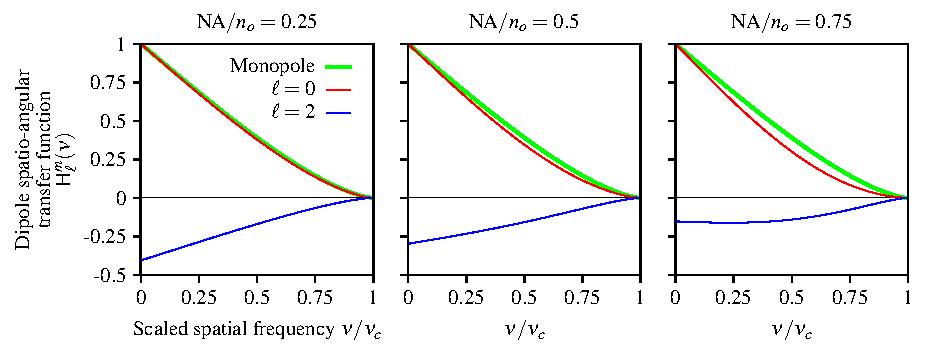
\includegraphics[scale=0.8]{../figures/paratfs/satf.pdf}
   \caption{Spatio-angular dipole transfer function as a function of the scaled
     spatial frequency $\nu/\nu_c$, the spherical harmonic degree $\ell$, and
     $\text{NA}/n_o$. When the numerical aperture is small the transverse
     dipoles contribute the most to the signal which gives rise to a positive
     $\ell=0$ component and a negative $\ell=2$ component. As the numerical
     aperture increases, the relative contribution of axial dipoles increases
     and the $\ell=2$ component becomes less negative. Additionally, we plot the
     monopole transfer function (\textcolor{green}{\textbf{green}}) and observe
     that the $\ell=0$ term is similar but not identical to the monopole
     transfer function, and this discrepancy increases with the numerical aperture.}
   \label{fig:dsatf}
 \end{figure}

 To demonstrate the spatio-angular transfer function, we simulate a set of
 equally spaced disks of fluorophores with varying radius and angular
 distributions
 \begin{align}
   f_{(ph4)}(r_x, r_y, \vartheta, \varphi) = \sum_{j=0}^3 \sum_{k=0}^3 \frac{1}{D_k^2}\Pi\left(\frac{1}{D_k}\sqrt{\left(r_x - j\right)^2 + \left(r_y - k\right)^2}\right)f_{\text{(cone)}}\left(\vartheta, \varphi; \frac{\pi}{2}, 0, \Delta_j\right),\label{eq:phantom4}
 \end{align}
 where $D_k = 0.15(1+k)\, \mu$m, and $\Delta_j = j\frac{\pi}{6}$. 
 
 Our first step towards calculating the irradiance pattern is to calculate the
 dipole spatio-angular spectrum given by the spatial Fourier transform of the dipole angular spectrum  
  \begin{align}
   \mathsf{F}_{\ell,(ph4)}^m(\nu_x, \nu_y) = \mc{F}_{\mbb{R}^2}\left\{\sum_{j=0}^3 \sum_{k=0}^3 \frac{1}{D_k^2}\Pi\left(\frac{1}{D_k}\sqrt{\left(r_x - j\right)^2 + \left(r_y - k\right)^2}\right)F_{\ell,\text{cone}}^m\left(\frac{\pi}{2}, 0, \Delta_j\right)\right\}.
  \end{align}
  We can plug the dipole spatio-angular spectrum into Eq. \eqref{eq:saft} to find
  the scaled irradiance as 
  \begin{align}
   g_{(ph4)}(r_x, r_y) = \mc{F}^{-1}_{\mbb{R}^2}\left\{\sum_{\ell m}\mathsf{H}_{\ell}^m(\nu_x, \nu_y)\mathsf{F}_{\ell,(ph4)}^m(\nu_x, \nu_y)\right\}.
  \end{align}

  In Fig. \ref{fig:ph4} we plot the phantom and scaled irradiance with the
  same imaging parameters as the previous sections. Small cone angles and small
  disks create relatively unique irradiance patterns, while increasing the cone
  angle or disk size creates increasingly similar irradiance patterns. 
  
  \begin{figure}[h]
 \centering
   \centering
   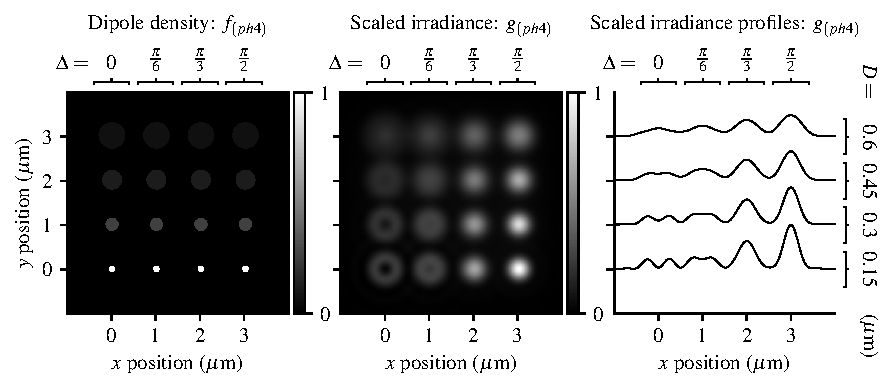
\includegraphics[scale=0.8]{../figures/paratfs/ph4.pdf}
   \caption{\textbf{Left:} A spatially and angularly dense phantom---uniformly
     spaced disks with varying size (increasing $D$ from bottom to top) and
     double cone half angle (increasing $\Delta$ from left to right)
     \textbf{Center:} Scaled irradiance for an imaging system with
     $\text{NA} = 0.75$, $\lambda = 500\,\text{nm}$, and $n_o = 1.33$ sampled at
     $20\times$ the Nyquist rate. \textbf{Right:} $x$ profiles through the
     scaled irradiance.}
   \label{fig:ph4}
 \end{figure}
 
\section{Discussion}\label{sec:discussion}
\subsection{When are dipole transfer functions necessary?}
Model mismatch can lead to biased estimates of the position and orientation of
fluorophores, so the most accurate fluorescence microscopy experiments will
always use dipole transfer functions over monopole transfer functions. The only
case when the dipole and monopole transfer functions match exactly is when the
dipoles are completely constrained to the transverse plane of a paraxial imaging
system.

However, in many practical situations noise will mask the effects of vector
optics and dipoles. If the fluorophores are rotationally unconstrained or there
are many randomly oriented fluorophores in a resolvable volume---common
situations in biological applications---then the effects of vector optics and
dipoles will be masked by noise in all but the highest-SNR regimes.

The dipole transfer functions are most broadly useful when the sample contains
fluorophores that are rotationally constrained. As rotational constraints
increase, the effects of vector optics and dipoles will become apparent in lower
SNR regimes.
 
\subsection{Alternative transfer functions}
Throughout this work we have used the spherical harmonic functions as a basis
for functions on the sphere, but there are other basis functions that can be
advantageous in some cases. Several works \cite{aguet2009, backer2014,
  brasselet2011, zhang2018, zhang2018-2} have used the second moments as basis
functions for the sphere because they arise naturally when computing the dipole
point spread function. These works use an alternative to the dipole angular
transfer function that uses the second moments as basis functions so the forward
model can be written as
\begin{align}
  g(\rd) = \sum_{j=1}^6 \int_{\mbb{R}^2}d\ro\, H_j(\rd - \ro)F_j(\ro),
\end{align}
where
\begin{align}
  H_j(\rd - \ro) &= \int_{\mbb{S}^2}d\so\, h(\rd - \ro, \so)Z_j(\so),\\
  F_j(\ro) &= \int_{\mbb{S}^2}d\so\, f(\ro, \so)Z_j(\so),
\end{align}
and $Z_j(\mh{s}) = \{s_x^2, s_y^2, s_z^2, s_xs_y, s_ys_z, s_xs_z\}$ are the
second moments. This formulation is similar to the dipole angular transfer
function approach because it can exploit the spatial sparsity of the sample, but
it does not require a cumbersome expansion of the dipole point spread function
onto spherical harmonics.

However, the spherical harmonics provide several advantages over the second
moments. First, the spherical harmonics form a complete basis for functions on
the sphere, while the second moments span a much smaller function space. The
usual approach to extending the span of the second moments is to use the fourth
(or higher) moments, but this extension requires a completely new set of basis
functions while the spherical harmonics can be extended by simply adding higher
order terms. Second, the spherical harmonics are orthonormal, which will allow
us to deploy invaluable tools from linear algebra---linear subspaces, rank, SVD,
etc.--- to analyze and compare microscope designs. Finally, using the spherical
harmonics provides access to a set of fast algorithms. The naive expansion of an
arbitrary discretized $N$ point spherical function onto spherical harmonics (or
second moments) requires a $\mc{O}(N^2)$ matrix multiplication, while pioneering
work by Driscoll and Healy \cite{driscoll1994} showed that the forward discrete
fast spherical harmonic transform can be computed with a $\mc{O}(N(\log N)^2)$
algorithm and its inverse can be computed with a $\mc{O}(N^{3/2})$ algorithm. To
our knowledge no similarly fast algorithms exist for expansion onto the
higher-order moments.

Zhenghao et. al. \cite{zhanghao2017} have used the circular harmonics to model
the orientation of dipoles. The circular harmonics are complete and orthogonal,
but they artificially restrict the reconstructed dipoles to the transverse
plane of the microscope---a rare situation in real experiments.

The diffusion magnetic resonance imaging community uses both the second moments
(or second-order tensor) basis functions \cite{basser1994} and the spherical
harmonic basis functions \cite{tournier2004}. Descoteaux et. al. have provided
an explicit transformation matrix to convert between these basis functions
\cite{descoteaux2006}.


\subsection{What determines the angular bandwidth?}
Spatial imaging systems have a spatial bandwidth that characterizes the highest
spatial frequency that the system can transfer between object and data space.
Similarly, angular imaging systems have an angular bandwidth that characterizes
the highest angular frequency that the system can transfer, but in the angular case
there are two different types of angular bandwidths that we call the $\ell$- and
$m$-bandwidth. The $\ell$-bandwidth can be interpreted in a similar way to the
spatial bandwidth---it characterizes the smallest angular features that the
imaging system can measure. The $m$-bandwidth does not have a direct analog in
the spatial domain---it characterizes the angular uniformity of the imaging
system. If the $\ell$- and $m$-bandwidths are equal then the imaging system can
be said to have an $\textit{isotropic angular bandwidth}$.

The spatial bandwidth of a fluorescence microscope is well known to be
$\nu_c = \frac{2\text{NA}}{\lambda}$. In other words, we can increase the
spatial resolution of a fluorescence microscope by increasing the NA of the
instrument or by choosing a fluorophore with a shorter emission wavelength.
Similarly, the angular bandwidth of a fluorescence microscope depends on both
the instrument and the choice of fluorophore.

The microscope we considered in this work has an $\ell$-bandwidth of
$\ell_c = 2$ and an $m$-bandwidth of $m_c = 0$, so it does not have an isotropic
angular bandwidth. In future work we will consider several approaches to
improving the angular bandwidths in detail, but we briefly mention that
non-paraxial microscopes, microscopes with polarizers in the illumination or
detection paths, and multiview microscopes all have higher angular bandwidths
than the microscope considered here.

The angular bandwidth is also fluorophore dependent. Monopoles emit light
isotropically so they have an $\ell$-bandwidth of $\ell_c = 0$, while dipoles
have an $\ell$-bandwidth of $\ell_c = 2$, and higher-order excitation and
detection moments will have even higher bandwidths. Multi-photon excitation and
other non-linear methods can also increase the $\ell$-bandwidth
\cite{brasselet2011}.

\subsection{Towards more realistic models}
The theoretical model we presented in this work is an extreme simplification of
a real microscope. We have ignored the effects of thick samples,
refractive-index mismatch, aberration, scattering, finite fluorescence
lifetimes, and interactions between fluorophores among others. Because of this
long list of unconsidered effects, real experiments will likely require
extensions of the models developed here.

The dipole pupil function provides the simplest way to create more realistic
models from the simple model in this paper. Phase aberrations can be added to
the dipole pupil function with Zernike polynomials, and refractive index
boundaries can be modeled by applying the work of Gibson and Lanni to the dipole
pupil function \cite{gibson89}. These additions will model phase aberrations,
but modeling polarization aberrations will also be necessary, and we anticipate
that vector Zernike polynomials and the Jones pupil \cite{zhao2007, xu2015,
  chipman1989} will be essential tools for modeling dipole imaging systems. We
plan to use the dipole pupil function to include the effects of non-paraxial
objectives, polarizers, and defocus in future papers of this series.

The dipole pupil function also provides an enormous set of design opportunities.
The dipole imaging problem may benefit from spatially varying diattenuating and
birefrigent masks---a much larger set of possibilities than the well-explored
design space of amplitude and phase masks. The dipole pupil function is a step
towards Green's tensor engineering \cite{agrawal2012}, and the dipole transfer
functions provide a strong framework for evaluating dipole imaging designs.

In the simple case considered here we focused on the emission path of the
microscope, but the excitation path is equally important. Complete models will
need to consider the spatio-angular dependence of excitation. Zhenghao et. al.
\cite{zhanghao2017} have taken steps in this direction by considering polarized
structured illumination microscopy. Rotational dynamics and the fluorescence
lifetime are also important to consider when incorporating models of the
excitation process \cite{lew2013, zhang2018, zhang2018-2}.

\subsection{Towards spatio-angular reconstructions}
We have focused on modeling the mapping between the object and the data in this
paper, but ultimately we are interested in reconstructing the object from the
data. Applying the monopole approximation simplifies the reconstruction problem
because both object and data space are $\mbb{L}_2(\mbb{R}^2)$, so we can
directly apply regularized inverse filters and maximum likelihood methods. The
dipole model expands object space to $\mbb{L}_2(\mbb{R}^2\times \mbb{S}^2)$, so
the inverse problem becomes much more challenging. In future work we will use
the singular value decomposition to find inverse filters, and we will consider
using polarizers and multiple views to increase the size of data space. 

\section{Conclusions}
Many models of fluorescence microscopes use the monopole and scalar
approximations, but complete models need to consider dipole and vector optics
effects. We have introduced several transfer functions that simplify the mapping
between the dipole density and the irradiance pattern on the detector, and we
have demonstrated these transfer functions by efficiently simulating a paraxial
fluorescence microscope. We found that the monopole and scalar approximations
are good approximations when the sample consists of unconstrained rotating
fluorophores or many randomly oriented fluorophores within a resolvable volume.
We also found that dipole and vector optics effects become larger as rotational
order increases, and in these cases the dipole transfer functions become
valuable tools.

\section*{Funding}
National Institute of Health (NIH) (R01GM114274, R01EB017293).

\section*{Acknowledgments}
We thank Kyle Myers, Harrison Barrett, Scott Carney, Luke Pfister, Jerome Mertz,
Sjoerd Stallinga, Mikael Backlund, Matthew Lew, Min Guo, Yicong Wu, Shalin
Mehta, Abhishek Kumar, Peter Basser, Marc Levoy, Michael Broxton, Gordon
Wetzstein, Hayato Ikoma, Laura Waller, Ren Ng, Tomomi Tani, Michael Shribak, Mai
Tran, Amitabh Verma, Xiaochuan Pan, Emil Sidky, Chien-Min Kao, Phillip Vargas,
Dimple Modgil, Sean Rose, Corey Smith, Scott Trinkle, and Jianhua Gong for
valuable discussions during the development of this work. TC was supported by a
University of Chicago Biological Sciences Division Graduate Fellowship, and PL
was supported by a Marine Biological Laboratory Whitman Center Fellowship.
Support for this work was provided by the Intramural Research Programs of the
National Institute of Biomedical Imaging and Bioengineering.

\section*{Disclosures}
The authors declare that there are no conflicts of interest related to this article.

\bibliography{paper}
\appendix
\section{Spherical harmonics and the spherical Fourier transform}\label{sec:sph}
The spherical harmonic function of degree $\ell$ and order $-\ell \leq m \leq \ell$
is defined as \cite{schaeffer2013}
\begin{align}
Y_\ell^m(\vartheta, \varphi) = \sqrt{\frac{2\ell+1}{4\pi}}\sqrt{\frac{(\ell-|m|)!}{(\ell+|m|)!}}P_\ell^m\left(\cos\vartheta\right)\exp(i m \varphi),
\end{align}
where $P_\ell^m(\cos\vartheta)$ are the associated Legendre polynomials with the
Condon-Shortley phase
\begin{align}
  P_\ell^m(x) = (-1)^m(1-x^2)^{|m|/2}\frac{d^{|m|}}{dx^{|m|}}P_\ell(x),
\end{align}
and $P_\ell(x)$ are the Legendre polynomials defined by the recurrence
\begin{align}
  P_0(x) &= 1,\\
  P_1(x) &= x,\\
  \ell P_\ell(x) &= (2\ell-1)xP_{\ell-1}(x) - (\ell-1)P_{\ell-2}(x). 
\end{align}
The spherical harmonics are orthonormal, which means that
\begin{align}
  \int_{\mbb{S}^2}d\mh{s}\, Y_\ell^m(\mh{s}){Y}_{\ell'}^{m'*}(\mh{s}) = \delta_{\ell\ell'}\delta_{mm'},
\end{align}
where $\delta_{\ell\ell'}$ denotes the Kronecker delta. The spherical harmonics form a
complete basis, so an arbitrary function on the sphere $f(\mh{s})$ can be
expanded into a sum of weighted spherical harmonic functions
\begin{align}
  f(\mh{s}) = \sum_{\ell=0}^{\infty}\sum_{m=-\ell}^{l}F_\ell^mY_\ell^m(\mh{s}).
\end{align}
We can find the spherical harmonic coefficients $F_\ell^m$ for a given function
using Fourier's trick---multiply both sides by $Y_\ell^{m*}(\mh{s})$,
integrate over the sphere, and exploit orthogonality to find that
\begin{align}
  F_\ell^m = \int_{\mbb{S}^2}d\mh{s}\, f(\mh{s})Y_\ell^{m*}(\mh{s}).
\end{align}
The coefficients $F_\ell^m$ are called the \textit{spherical Fourier transform}
of a spherical function.

\section{Relationships between special functions} \label{sec:special}
Our first task is to show that 
\begin{align}
  i^{n}\left\{\substack{
  \text{exp}(in\phi_r)\\
    \cos(n\phi_r)\\
    \sin(n\phi_r)
  }\right\}\text{jinc}_{n}(r) &\stackrel{\mathcal{F}_{\mbb{R}^2}}{\longrightarrow}   (2\nu)^{n}\left\{\substack{
    \text{exp}(in\phi_{\nu})\\
    \cos(n\phi_{\nu})\\
    \sin(n\phi_{\nu})
  }\right\}\Pi(\nu). \label{eq:jincrect3}
  \end{align}
  Writing the inverse Fourier transform in polar coordinates yields
  \begin{align}
    =2^n\int_0^{1/2}d\nu\, \nu^{n+1}\int_0^{2\pi}d\phi_\nu\left\{\substack{
    \text{exp}(in\phi_{\nu})\\
    \cos(n\phi_{\nu})\\
    \sin(n\phi_{\nu})
  }\right\}\text{exp}[2\pi i\nu r\cos(\phi_\nu - \phi_r)].
  \end{align}
  The azimuthal integral can be evaluated in terms of an $n^{th}$ order Bessel
  function (for the complex case see \cite[ch. 4.111]{barrett2004}).
  \begin{align}
    =2^n 2\pi i^n \left\{\substack{
    \text{exp}(in\phi_{r})\\
    \cos(n\phi_r)\\
    \sin(n\phi_r)
  }\right\}\int_0^{1/2}d\nu\, \nu^{n+1}J_n(2\pi\nu r).
  \end{align}
  We can use the following identity \cite[ch.~6.561-5]{gradshteyn2007}
  \begin{align}
    \int_0^1 du\, u^{n + 1}J_{n}(au) = a^{-1}J_{n + 1}(a)
  \end{align}
  with a change of variable $u = 2\nu$ to find the final result
  \begin{align}
    &=2^n 2\pi i^n \left\{\substack{
    \text{exp}(in\phi_{r})\\
    \cos(n\phi_r)\\
    \sin(n\phi_r)
  }\right\}\int_0^{1}\frac{du}{2}\, \left(\frac{u}{2}\right)^{n+1}J_n(\pi u r)
    =i^n \left\{\substack{
    \text{exp}(in\phi_{r})\\
    \cos(n\phi_r)\\
    \sin(n\phi_r)
  }\right\}\frac{J_{n+1}(\pi r)}{2r}
    =i^n \left\{\substack{
    \text{exp}(in\phi_{r})\\
    \cos(n\phi_r)\\
    \sin(n\phi_r)
  }\right\}\text{jinc}_{n}(r).
  \end{align}

\begin{figure}[h]
 \centering
   \centering
   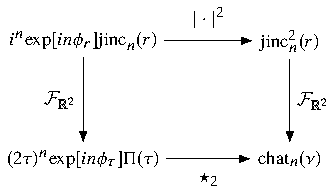
\includegraphics[width = 0.45\textwidth]{../figures/special/special.pdf}
   \caption{The relationships between special functions. The chat functions are
     defined as the two-dimensional Fourier transform of the squared jinc
     functions, and they can be calculated with the two-dimensional complex
     autocorrelations (denoted by $\star_2$) of the complex-weighted rectangle
     functions.}
   \label{fig:special}
 \end{figure}


We can use the relationship in Eq. \eqref{eq:jincrect3} to express the chat
functions in terms of a complex autocorrelation---see the diagram in Fig. \ref{fig:special}. Starting with the definition of
the $n^{th}$-order chat function
\begin{align}
  \text{chat}_{n}(\nu) = \int_{\mbb{R}^2}d\mb{r}\, \text{jinc}_{n}^2(|\mb{r}|)\, \text{exp}\left[-2\pi i\mb{r}\nu\right],  \label{eq:ftA}
\end{align}
we can rewrite the integrand in terms of the absolute square of a simpler
function with a known Fourier transform
\begin{align}
  \text{chat}_{n}(\nu) = \int_{\mbb{R}^2}d\mb{r}\, |t_n(\mb{r})|^2\, \text{exp}\left[-2\pi i\mb{r}\nu\right].  \label{eq:ftB}
\end{align}
\begin{align}
  t_n(\mb{r}) = i^n\text{exp}[in\phi_r]\text{jinc}_{n}(r).
\end{align}
Now we can apply the autocorrelation theorem to rewrite the Fourier transform as
\begin{align}
  \text{chat}_{n}(\nu) = \int_{\mbb{R}^2}d\bs{\tau}\, T_n(\bs{\tau})T^*_n(\bs{\tau} - \nu), \label{eq:autocorr}
\end{align}
where the function to be autocorrelated can be found with the help of Eq. \eqref{eq:jincrect3}
\begin{align}
  T_n(\bs{\tau}) = \int_{\mbb{R}^2}d\mb{r}\, t_n(\mb{r})\text{exp}\left[-2\pi i\mb{r}\cdot\bs{\tau}\right] = (2\tau)^n\text{exp}[in\phi_\tau]\Pi\left(\tau\right). \label{eq:tau}
\end{align}
It will be more convenient to set up the autocorrelation in Cartesian coordinates 
\begin{align}
  T_n(\bs{\tau}) &= 2^n(\tau_x + i\tau_y)^{n}\Pi\left(\sqrt{\tau_x^2 + \tau_y^2}\right). \label{eq:tn}
\end{align}
Plugging Eq. \eqref{eq:tn} into Eq. \eqref{eq:autocorr} gives
\begin{align}
  \text{chat}_{n}(\nu) = 4^n\int_{\mbb{R}^2}d\bs{\tau}\, (\tau_x^2 + \tau_y^2 - \nu\tau_x)^{n}\Pi\left(\sqrt{\tau_x^2 + \tau_y^2}\right)\Pi\left(\sqrt{(\tau_x - \nu)^2 + \tau_y^2}\right).
\end{align}
We can interpret the autocorrelation as an integral over a region of overlap
between a circle centered at the origin and a circle shifted to the right by
$\nu$ (a geometric lens). Using the construction in Fig. \ref{fig:geometry} we
can express this region as
\begin{align}
  \text{chat}_{n}(\nu) = 4^{n+1}\Bigg[&\int_0^{1/2}\tau d\tau\int_0^{\cos^{-1}\nu}d\phi_{\tau}(\tau^2 - \nu\tau\cos\phi_{\tau})^{n} -\nonumber \\ &\int_{0}^{\nu/2}d\tau_x\int_0^{\frac{\tau_x}{\nu}\sqrt{1 - \nu^2}}d\tau_y(\tau_x^2 + \tau_y^2 - \nu\tau_x)^{n}\Bigg]\Pi\left(\frac{\nu}{2}\right).
\end{align}
\begin{figure}[h]
 \centering
   \centering
   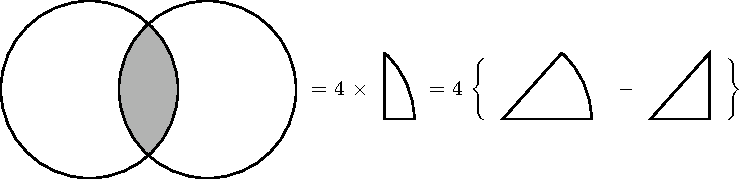
\includegraphics[width = 1.0\textwidth]{../figures/autocorrelation/autocorrelation.pdf}
   \caption{Geometric construction for evaluating the autocorrelation. We need
     to integrate over the overlapping region of two circles with radius $1/2$
     and distance $\nu$ between their centers. The region is four times the
     difference in area between a sector of angle $\cos^{-1}(\nu)$ and radius
     $1/2$ and a right triangle with base $\nu/2$ and hypotenuse $1/2$.}
   \label{fig:geometry}
 \end{figure}

For $n=0$:
\begin{align}
  \text{chat}_0(\nu) &= 4\left[\int_0^{1/2}\tau d\tau\int_0^{\cos^{-1}\nu}d\phi_{\tau} - \int_{0}^{\nu/2}d\tau_x\int_0^{\frac{\tau_x}{\nu}\sqrt{1 - \nu^2}}d\tau_y\right]\Pi\left(\frac{\nu}{2}\right),\\
  \text{chat}_0(\nu) &= \frac{1}{2}\left[\cos^{-1}|\nu| - |\nu|\sqrt{1 - \nu^2}\right]\Pi\left(\frac{\nu}{2}\right),
\intertext{which is a well-known result \cite{goodman1996, mertz2009, bracewell2004}. For $n=1$:}
  \text{chat}_1(\nu) &= 16\Bigg[\int_0^{1/2}\tau d\tau\int_0^{\cos^{-1}\nu}d\phi_{\tau}(\tau^2 - \nu\tau\cos\phi_{\tau}) - \nonumber\\ &\qquad\quad\int_{0}^{\nu/2}d\tau_x\int_0^{\frac{\tau_x}{\nu}\sqrt{1 - \nu^2}}d\tau_y\, (\tau_x^2 + \tau_y^2 - \nu\tau_x)\Bigg]\Pi\left(\frac{\nu}{2}\right),\\
  \text{chat}_1(\nu) &= \frac{1}{2}\left[\cos^{-1}|\nu| - |\nu| (3 - 2\nu^2)\sqrt{1 - \nu^2}\right]\Pi\left(\frac{\nu}{2}\right). 
\end{align}

\section{Spherical Fourier transform of a double cone}\label{sec:cone}
In this appendix we evaluate the spherical Fourier transform of a
normalized double-cone angular distribution with central direction $\mh{s}'$ and
cone half-angle $\Delta$
\begin{align}
  f_{\text{(cone)}}(\mh{s}; \mh{s}', \Delta) = \frac{1}{4\pi(1 - \cos\Delta)}\Pi\left(\frac{\mh{s}\cdot\mh{s}'}{2\cos\Delta}\right). \label{eq:doublecone}
\end{align}
The spherical Fourier transform is
\begin{align}
  F_{\ell\text{(cone)}}^m(\mh{s}', \Delta) = \int_{\mbb{S}^2}d\mh{s}\, f_{\text{(cone)}}(\mh{s}; \mh{s}', \Delta)Y_\ell^{m*}(\mh{s}).
\end{align}

The limits of integration will be difficult to find unless we change coordinates
to exploit the axis of symmetry $\mh{s}'$. Since the spherical function is
rotationally symmetric about $\mh{s}'$ we can rotate the function so that the axis of
symmetry is aligned with $\mh{z}$ and multiply by $\sqrt{\frac{4\pi}{2l+1}}Y_\ell^{m*}(\mh{s}')$ to account for the rotation \cite{ramamoorthi2005}
\begin{align}
    F_{\ell\text{(cone)}}^m(\mh{s}', \Delta) = \sqrt{\frac{4\pi}{2l+1}}Y_\ell^{m*}(\mh{s}')\int_{\mbb{S}^2}d\mh{s}\, f_{\text{(cone)}}(\vartheta; \mh{z}, \Delta)Y_\ell^0(\mh{s}). 
\end{align}
In this coordinate system the double cone is independent of the azimuthal angle,
so we can evaluate the azimuthal integral and express the function in terms of an
integral over $\vartheta$:
\begin{align}
    F_{\ell\text{(cone)}}^m(\mh{s}', \Delta) = 2\pi Y_\ell^{m*}(\mh{s}')\int_{0}^\pi d\vartheta\, \sin\vartheta f_{\text{(cone)}}(\vartheta; \mh{z}, \Delta)P_\ell(\cos\vartheta). 
\end{align}
The function $f_{\text{(cone)}}(\vartheta; \mh{z}, \Delta)$ is only non-zero on
the intervals $\vartheta \in [0, \Delta]$ and
$\vartheta \in [\pi - \Delta, \pi]$ so
\begin{align}
    F_{\ell\text{(cone)}}^m(\mh{s}', \Delta) = \frac{Y_\ell^{m*}(\mh{s}')}{2(1 - \cos\Delta)}\left[\int_{0}^\Delta d\vartheta\, \sin\vartheta P_\ell(\cos\vartheta) + \int_{\pi - \Delta}^\pi d\vartheta\, \sin\vartheta P_\ell(\cos\vartheta)\right]. 
\end{align}
Applying a change of coordinates with $u = \cos\vartheta$ yields
\begin{align}
    F_{\ell\text{(cone)}}^m(\mh{s}', \Delta) = \frac{Y_\ell^{m*}(\mh{s}')}{2(1 - \cos\Delta)}\left[\int_{\cos\Delta}^1 d\vartheta\, P_\ell(u) + \int_{-1}^{-\cos\Delta} d\vartheta\, P_\ell(u)\right]. 
\end{align}
The Legendre polynomials $P_\ell(u)$ are even (odd) on the interval [-1, 1] when
$\ell$ is even (odd), so the pair of integrals will be identical when $\ell$ is
even and cancel when $\ell$ is odd. For even $\ell$,
\begin{align}
  F_{\ell\text{(cone)}}^m(\mh{s}', \Delta) = \frac{Y_\ell^{m*}(\mh{s}')}{1 - \cos\Delta}\int_{\cos\Delta}^1 d\vartheta\, P_\ell(u).
\end{align}
The integral evaluates to \cite[ch.~7.111]{gradshteyn2007}
\begin{align}
  \int_{\cos\Delta}^1 d\vartheta\, P_\ell(u) =
\begin{cases}
  1 - \cos\Delta\,, &\ell = 0\,,\\
  \sin\Delta\, P_l^{-1}(\cos\Delta)\,, &\text{else},
\end{cases}
\end{align}
where $P_l^{-1}(\cos\Delta)$ is the associated Legendre polynomial with order
$m=-1$, not an inverse Legendre polynomial. Bringing everything together
\begin{align}
  F_{\ell\text{(cone)}}^m(\mh{s}', \Delta) =
  \begin{cases}
    \sqrt{1/(4\pi)}, & \ell = 0,\\
    0, & \ell\, \text{odd},\\
    Y_\ell^{m*}(\mh{s}')\cot\left(\frac{\Delta}{2}\right)P_l^{-1}(\cos\Delta), & \ell > 0\,\, \text{even}.
  \end{cases}
\end{align}

\end{document}
